\documentclass[xcolor=table]{beamer}
\usepackage[utf8]{inputenc}
\usepackage[british]{babel}
\usepackage[super]{nth}
%\usetheme{Boadilla}
%\usecolortheme{rose}
%\usecolortheme{crane}
%\usefonttheme{structuresmallcapsserif}
%\setbeamertemplate{navigation symbols}{}

\definecolor{Main}{rgb}{0.74, 0.13, 0.19}
\definecolor{Accent1}{rgb}{0.76,0.36,0.13}
\definecolor{Accent2}{rgb}{0.54,0.1,0.4}

\mode<presentation>{\usetheme{ilm}}
%\usecolortheme{rose}
%\useinnertheme[shadow]{circles}
%\usecolortheme{whale}
%\useoutertheme{infolines}

%\usecolortheme[named=Accent1]{structure}




%\setbeamerfont{page number in head/foot}{size=\large}
%\setbeamercolor{page number in head/foot}{fg=Main}
%% page/total
%%\setbeamertemplate{footline}[frame number]
%% pas de total
%\setbeamertemplate{footline}{%
%    	\hfill%
%	\usebeamercolor[fg]{page number in head/foot}%
%	\usebeamerfont{page number in head/foot}%
%	\insertframenumber\kern1em\vskip2pt%
%}
%
%\setbeamersize{text margin left=1em}
%\setbeamersize{text margin right=1em}

\usepackage[overlay,absolute]{textpos}
\setlength{\TPHorizModule}{10mm}
\setlength{\TPVertModule}{\TPHorizModule}
\textblockorigin{10mm}{10mm} % start everything near the top-left corner
\setlength{\parindent}{0pt}

%font
\usepackage[T1]{fontenc}
\usepackage{times}
%\usepackage[oldstylenums]{kpfonts}

%\include{macros}


%proper math and math symbols
%\usepackage{amsmath}
\usepackage{amssymb}

\usepackage{datenumber,fp}

\usepackage[separate-uncertainty = true]{siunitx}

\usepackage{tabu}
\usepackage{multirow}
\usepackage{booktabs}

% Allow the usage of graphics (.jpg, .png, etc.) in the document
\usepackage{graphicx}
\usepackage{tikz}
\usetikzlibrary{arrows,shapes,backgrounds, calc, positioning, topaths,chains, intersections, decorations.markings, decorations.text, shapes.geometric, matrix,patterns,mindmap}
%\usetikzlibrary{positioning, patterns,topaths,chains,matrix}

\usepackage{pgfplots}
\usepackage{pgfplotstable}
\pgfplotsset{compat=1.9}
\usepgfplotslibrary{groupplots}
\usepgfplotslibrary{external}
\makeatletter
\newcommand*{\overlaynumber}{\number\beamer@slideinframe}
\tikzset{
  beamer externalizing/.style={%
    execute at end picture={%
      \tikzifexternalizing{%
        \ifbeamer@anotherslide
        \pgfexternalstorecommand{\string\global\string\beamer@anotherslidetrue}%
        \fi
      }{}%
    }%
  },
  external/optimize=false
}
\let\orig@tikzsetnextfilename=\tikzsetnextfilename
\renewcommand\tikzsetnextfilename[1]{\orig@tikzsetnextfilename{#1-\overlaynumber}}
\makeatother

\tikzset{every picture/.style={beamer externalizing}}
\tikzexternalize
\tikzsetexternalprefix{fig_presentation/}
%\tikzset{external/optimize=false}
%\tikzset{external/force remake}


%link or play movies
\usepackage{multimedia}



%beamer related package

\usepackage{todonotes}
\presetkeys{todonotes}{inline}{}

\tikzset{onslide/.code args={<#1>#2}{%
  \only<#1>{\pgfkeysalso{#2}} %
}}%


%bibliography
\usepackage[style=authoryear-comp, language=british,eprint=false, url=false, doi=false, sortcites=true, sorting=none, isbn=false, firstinits=true,maxcitenames=6]{biblatex}
%minimal citations
\AtEveryCitekey{%
	\clearfield{title}
	\clearfield{pages}
	\clearfield{volume}
	\clearfield{number}
	\clearfield{month}}
\newcommand{\myfullcite}[1]{{\scriptsize\fullcite{#1}}}
\renewbibmacro{in:}{%
  \ifentrytype{article}{}{%
  \printtext{\bibstring{in}\intitlepunct}}}
%\bibliography{biblio}


\newcolumntype{P}[1]{>{\raggedright}p{#1}}

\institute[iLM]{iLM, Univ. Claude Bernard Lyon 1 and CNRS, France}
\title[crystal gel]{A novel route to the spontaneous formation of porous crystals via viscoelastic phase separation}
\author[M. Leocmach]{Mathieu Leocmach}
\date{30 June 2016}
\titlegraphic{
	\begin{tabu}{X[c]X[c]X[c]}
		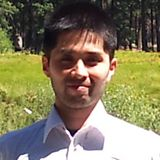
\includegraphics[height=3\baselineskip]{presentation/Tsurusawa}&
		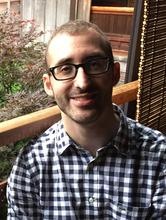
\includegraphics[height=3\baselineskip]{presentation/John}&
		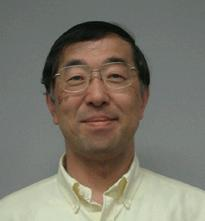
\includegraphics[height=3\baselineskip]{presentation/Tanaka}\\
		Hideyo Tsurusawa & John Russo & Hajime Tanaka\\
		U. Tokyo & U. Bristol & U. Tokyo\\
	\end{tabu}
	
	%\vfill
	%\includegraphics[height=2\baselineskip]{logo_ens-lyon}\quad
	%\includegraphics[height=2\baselineskip]{logo_ums_grand}\quad
	%\includegraphics[height=2\baselineskip]{../../Yaourt/CNRSfilaire-Q}\quad
	%\includegraphics[height=2\baselineskip]{CRPP}\quad
	%\includegraphics[height=2\baselineskip,clip=true, trim=6mm 14mm 6mm 0]{NEW-Logo-ERC-OUTLINE}
	}


\newlength{\mylength}

%\includeonly{creep_beamer}

\begin{document}
\tikzset{every mark/.append style={scale=0.8}}
\pgfplotsset{every axis/.append style={footnotesize}}

\pgfplotscreateplotcyclelist{earthy}{%
{red!40!black,mark=o},
{red!60!black,mark=triangle, every mark/.append style={rotate=180}},
{red!80!black,mark=square},
{red,mark=triangle},
{red!80!yellow, mark=diamond},
red!60!yellow,
red!40!yellow,
}

\AtBeginSection[]{
	\addtocounter{framenumber}{-1}
	\begin{frame}[plain]
		\tableofcontents[currentsection, hideothersubsections]
	\end{frame}
}

\begin{frame}{\pgfuseimage{cnrs-logo}\hspace*{0.3cm}\pgfuseimage{ucbl-logo}}%[plain]
	\titlepage
\end{frame}

\setcounter{framenumber}{0}

\begin{frame}{Crystallisation}
	\tikzsetnextfilename{whyx}%
	\begin{tikzpicture}
\node[text width=0.25\textwidth, anchor=base west] (process){
Crystallisation
\begin{itemize}
\item nucleation
\item growth
\end{itemize}};

\node[anchor=base east] (prop) at (\textwidth,0){
Properties
};

\node[text width=0.39\textwidth, anchor=base] (x) at ($(process.base east)!0.5!(prop.base west)$){
Crystalites
\begin{itemize}
\item polymorph type
\item shape
\item spatial arrangement
\item size distribution
\end{itemize}};


% 
\node[above left=3em and 0 of prop.east] (np){natural processes};
\node[below left=8em and 0 of prop.east] (tech){technological applications};

\begin{scope}[->,ultra thick, ilmcolor]
\draw (process.base east) +(0,0.3em) -- ($(x.base west)+(0,0.3em)$);
\draw (x.base) +(0,0.3em) -- ($(prop.base west)+(0,0.3em)$);
\draw (prop) -- (np.south-|prop);
\draw (prop) -- (tech.north-|prop);
\end{scope}
\end{tikzpicture}
	
	\begin{block}{Nucleation}
	\begin{itemize}
		\item 10-1000 molecules $\rightarrow$ difficult to observe
		\item classical nucleation theory (CNT): fluid $\xrightarrow{\text{1 step}}$ crystal
	\end{itemize}
	\end{block}
\end{frame}
	
\begin{frame}{Let it snow!}
	\hfill Wegener-\alert{Bergeron}-Findeisen \alert{process}
	\begin{columns}[b]
	\column{0.4\textwidth}
	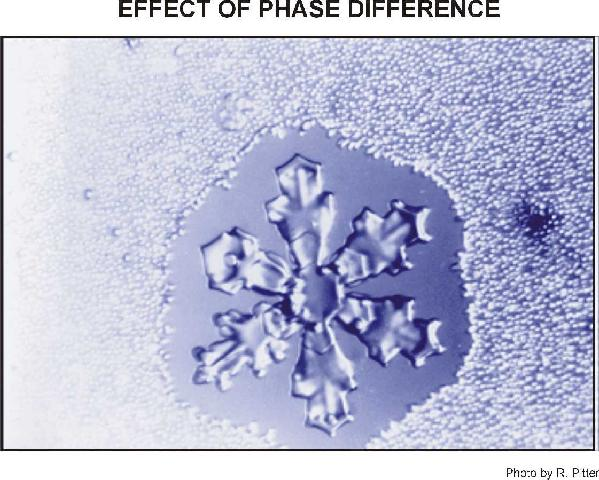
\includegraphics[width=\textwidth,clip=true,trim=0 0 0 1cm]{presentation/Pitter1.jpg}
	
	\vspace{1em}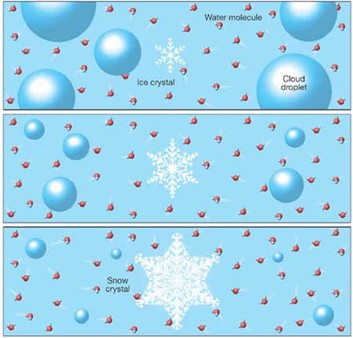
\includegraphics[width=\textwidth]{presentation/bergeron.jpg}
	\column{0.40\textwidth}
	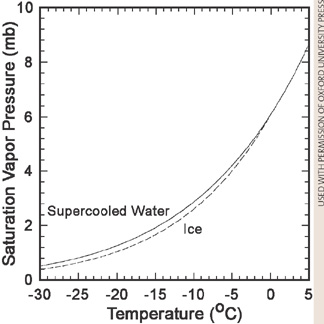
\includegraphics[width=\textwidth,clip=true,trim=0 0 0.8mm 0]{presentation/queries-figure-1.jpg}
	
	\vspace{1em}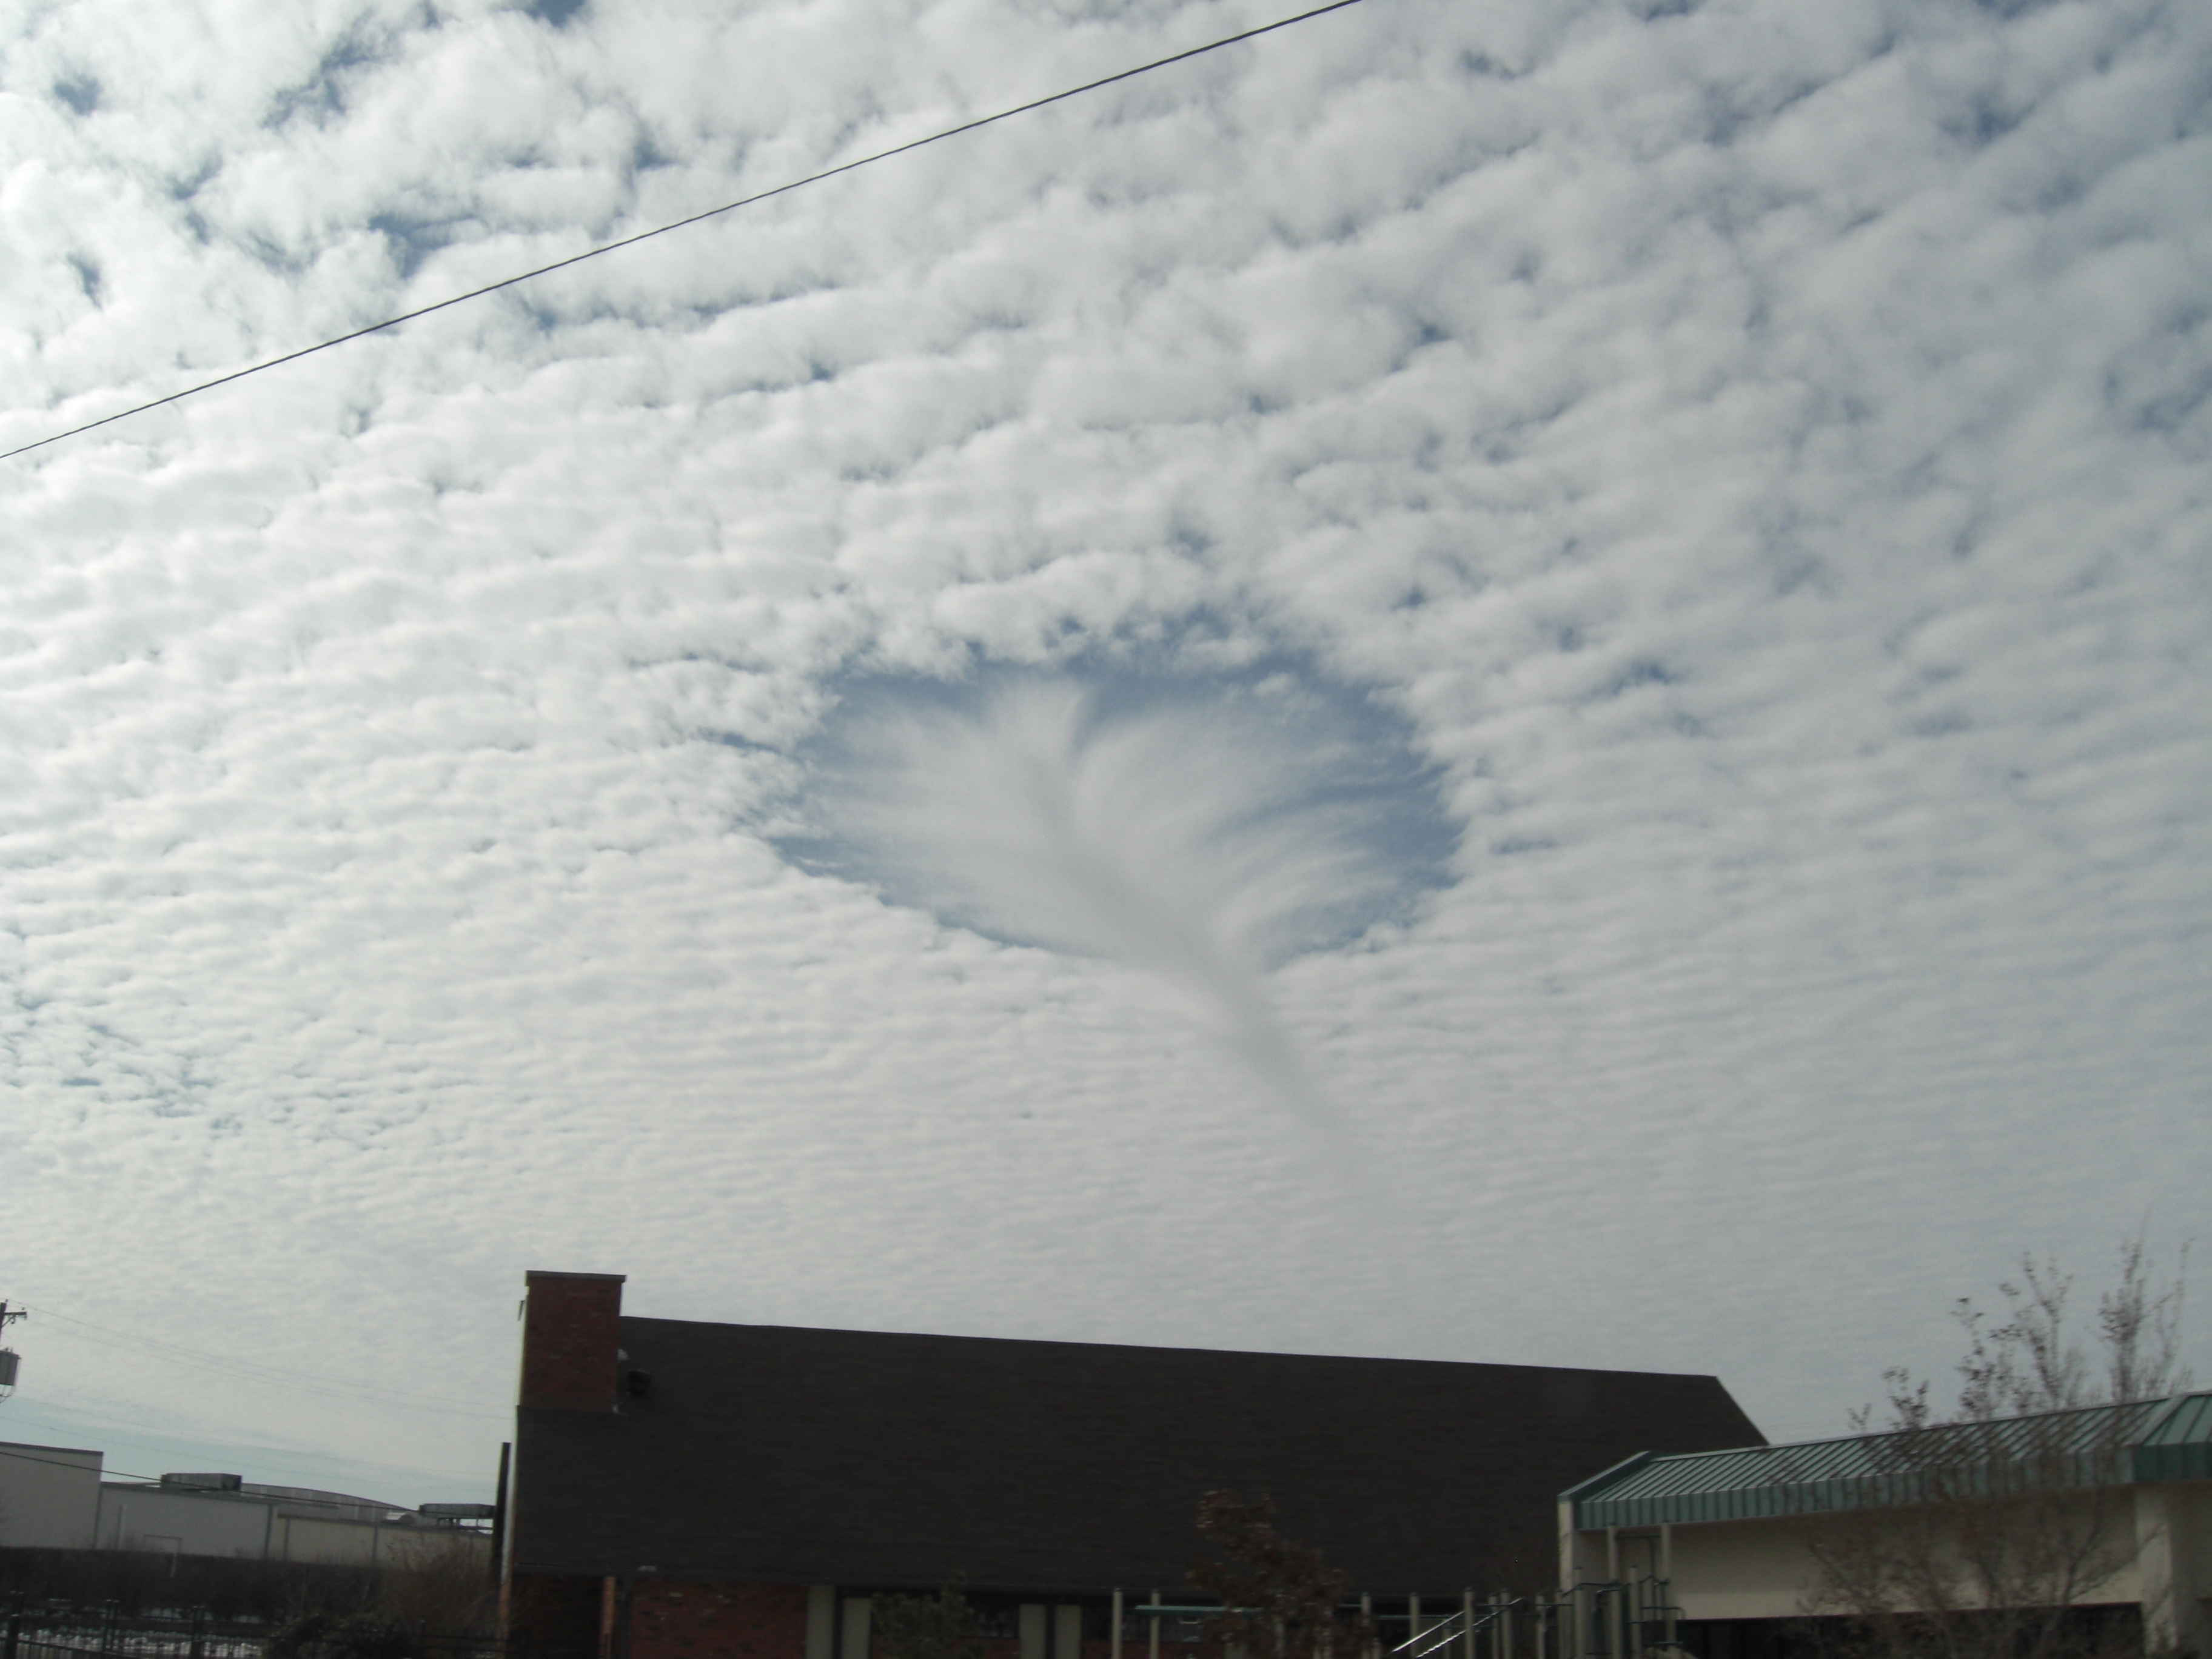
\includegraphics[width=\textwidth]{presentation/OKC-Fallstreak.jpg}
	\end{columns}
\end{frame}


\begin{frame}{Big atoms: Colloid + Polymer}
	\begin{columns}
	\column{0.5\textwidth}
	\begin{itemize}
		\item visible, trackable
		\item tunable interactions
	\end{itemize}
	\medskip
	\tikzsetnextfilename{interactions}%
	\begin{tikzpicture}[every node/.style={font=\footnotesize}]
		\let\mrad\relax
		\newlength\mrad
		\setlength{\mrad}{1em}
		
		
		%schemas interactions
		
		%repulsion
		\begin{scope}[xshift=2\mrad]
		\node[circle, inner sep=0, minimum width=4\mrad, inner color=Main, outer color=white]  (puri) {}; 
		\foreach \x in {0,30,...,330}{
			\draw[decoration={random steps,segment length=0.1\mrad, amplitude=0.08\mrad},decorate] (0,0) -- (\x:1\mrad);
		}
		\fill[gray, radius=0.8\mrad] circle;
		\foreach \x in {15,75,...,315}{
			\node[Accent2, font=\tiny] at (\x:0.6\mrad) {+};
		}
		\end{scope}
		
		%spheres collantes
		\begin{scope}[xshift=\textwidth-2.5\mrad]
		\node[draw,circle, inner sep=0, minimum width=2.5\mrad, green!50!black, dashed]  (colli) {}; 
		\draw[green!50!black, radius=1.25\mrad, dashed] (1.6\mrad,0) circle;
		\fill[gray, radius=0.8\mrad] circle;
		\fill[gray, radius=0.8\mrad] (1.6\mrad,0) circle;
		\end{scope}
		
		\path (puri) -- (colli) coordinate[midway] (m);
		
		%spheres dures
		\begin{scope}[shift=(m)]
		\node[circle, inner sep=0, minimum width=2.2\mrad, inner color=Main, outer color=white]  (duri) {}; 
		\foreach \x in {0,30,...,330}{
			\draw[decoration={random steps,segment length=0.1\mrad, amplitude=0.08\mrad},decorate] (0,0) -- (\x:1\mrad);
		}
		\fill[gray, radius=0.8\mrad] circle;
		\foreach \x in {15,75,...,315}{
			\node[Accent2, font=\tiny] at (\x:0.6\mrad) {+};
		}
		\end{scope}
		
		%fleches
		\draw[->] (puri) -- (duri) node[midway,above,font=\footnotesize]{ions};
		\draw[->] (duri) -- (colli)node[midway, above,font=\footnotesize]{PS};
		% \draw[->] (puri) -- (ps) -- (depli);
		
		
		%titres
		\node[text width=6em,anchor=base west, inner xsep=0] (pur) at (puri.west|-puri.north) {repulsion};
		
		\node[text width=6em,anchor=base, align=center] (dur) at (duri|-pur.base) {hard};
		
		\node[text width=6em, anchor=base east, inner xsep=0,xshift=1.5\mrad, align=right] (coll) at (colli.east|-pur.base) {depletion};
	\end{tikzpicture}
	\begin{block}{Various phases}
		\begin{itemize}
			\item triple coexistence\\
			\textit{\footnotesize Poon PRL 1999}
			\item gas-liquid metastable\\\hfill to gas-crystal
		\end{itemize}
	\end{block}
	\column{0.5\textwidth}
	\vspace{0.5\baselineskip}
	\hfill\tikzsetnextfilename{sedim_glx}%
	\begin{tikzpicture}
		\node[inner sep=0] (sedim){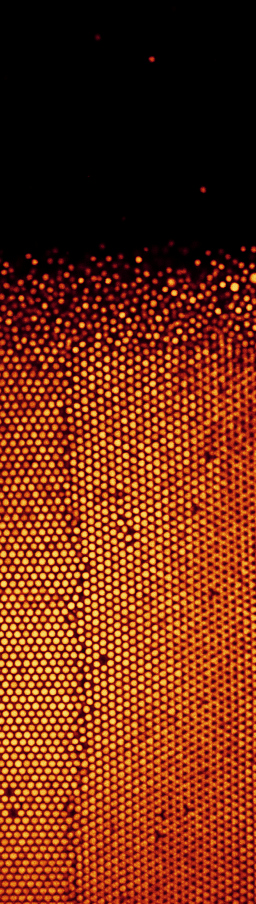
\includegraphics[height=17\baselineskip, clip=true, trim=0 250 0 0]{presentation/sedim_gas_liq_crystal_p.png}};
		\path[every node/.style={left}] (sedim.north west) -- (sedim.south west) node[pos=0.1] {gas} node[pos=0.45] {liquid} node[pos=0.8] {crystal} node[pos=0.15, ilmorange, font=\itshape] {low viscosity} node[pos=0.5, ilmcolor, font=\itshape] {high viscosity};
		\node[anchor=north east, font=\scriptsize, inner sep=1pt] at (sedim.south east) {Paddy Royall};
	\end{tikzpicture}
	\end{columns}
\end{frame}

\begin{frame}{Gel formation}
		\begin{columns}
		\column{0.5\textwidth}
		\vspace{\baselineskip}
		\tikzsetnextfilename{phdiagth}%
		\begin{tikzpicture}[
			every axis/.style={
			xlabel absolute, every axis x label/.append style={anchor=base, yshift=-0.5em},
			ylabel absolute, every axis y label/.append style={anchor=base, yshift=-0.5em}
			}]
% 		\pgfplotscreateplotcyclelist{samples}{%
% 		blue,mark=square*,\\%
% 		cyan,mark=square\\%
% 		red, thick, mark=*\\%
% 		red!65!yellow, mark=otimes\\%
% 		red!30!yellow, mark=oplus\\%
% 		red!65!black, mark=o\\%
% 		}%
		\begin{groupplot}[
			group style={
					group name=g, group size=1 by 2,
					horizontal sep=4em,
					vertical sep=0.5em,
					x descriptions at=edge bottom,
				},
			%cycle list name=samples,
			width=\textwidth,
			%height=0.5\linewidth,
			axis on top,
		]
		\nextgroupplot[
			ylabel={attraction},
			xmin=0,xmax=0.74,
			ymin=0, ymax=2400, %ytick={0,0.5,...,2},
			mark options={solid}
			]
			\addplot[fill=lightgray!50, no marks, draw=none] file {res_fluidcrystal_f.phd} node[above right] at (rel axis cs:0,0) {fluid} -- (rel axis cs:0,0) coordinate (O) \closedcycle;
			\addplot[fill=lightgray!50, no marks, draw=none] file {res_fluidcrystal_x.phd} node[above left, inner ysep=0, inner xsep=1pt] (x) at (rel axis cs:1,0) {crystal}  -| (rel axis cs:1,0) \closedcycle;
			\addplot[black, dashed,no marks] file {res_gasliquid_sg.phd};% node[diamond, fill, inner sep=2pt] at (current plot begin){};
			\addplot[black, dashed,no marks] file {res_gasliquid_sl.phd};
			\addplot[black, no marks] file {res_gasliquid_bl.phd} node[pos=0.5,sloped,below,ilmcolor] (l) {liquid};
			\addplot[black, no marks] file {res_gasliquid_bg.phd} node[pos=0.1,sloped,below,ilmorange] {gas};
			
			\node at (axis cs:0.35,2000) {g-l spinodal};
			\draw[<->, thick, dotted] (l) -- (l -| O) node[pos=0.5,fill] {};
			%glass
			\only<2>{\addplot[pattern=crosshatch, pattern color=ilmcolor,no marks, draw=none] coordinates {(0.56,0) (0.6,500) (0.56,2400)}  -- (rel axis cs:1,1)  \closedcycle;}
			
	
		\nextgroupplot[
			xlabel={colloid volume fraction}, ylabel={P concent.  (\si{\milli\gram/\gram})},
			xmin=0,xmax=0.74,
			ymin=0, ymax=1.9, ytick={0,0.5,...,2},
			mark options={solid}
			]
			\addplot[fill=lightgray!50, no marks, draw=none] file {fluidcrystal_f.phd} node[above right] at (rel axis cs:0,0) {fluid} -- (rel axis cs:0,0) \closedcycle;
			\addplot[fill=lightgray!50, no marks, draw=none] file {fluidcrystal_x.phd} %node[above left, inner ysep=0, inner xsep=1pt] (x) at (rel axis cs:1,0) {Crystal}  
-| (rel axis cs:1,0) \closedcycle;
			\addplot[black, dashed,no marks] file {gasliquid_sg.phd};% node[diamond, fill, inner sep=2pt] at (current plot begin){};
			\addplot[black, dashed,no marks] file {gasliquid_sl.phd};
			\addplot[black, no marks] file {gasliquid_bl.phd} node[pos=1,sloped,below,ilmcolor] (l) {liquid};
			\addplot[black, no marks] file {gasliquid_bg.phd} node[pos=0.3,sloped,below,ilmorange] {gas};
			\draw[<->, thick, dotted] (l.north) -- (rel axis cs:0,1) node[pos=0.5,fill] {};
			%glass
			\only<2>{\addplot[pattern=crosshatch, pattern color=ilmcolor,no marks, draw=none] coordinates {(0.56,0) (0.6,0.125) (0.56,2)}  -- (rel axis cs:1,1)  \closedcycle;}
			
			%\draw[->] (x.base) --(rel axis cs:0.98,0.01);
		\end{groupplot}
		\node[anchor=north west, rotate=90, inner xsep=0,lightgray] (x) at (g c1r2.south east) {crystal};
		%\draw(g c1r1.outer south west) -- +(\textwidth,0);
		\end{tikzpicture}
		\column{0.5\textwidth}
		%Small polymer/colloid size ratio
		\structure{Dynamic assymetry}
		\tikzsetnextfilename{vps}%
		\begin{tikzpicture}
	\draw[->] (0,0) -- +(\textwidth,0) node[pos=0.05, label=-90:\textcolor{ilmorange}{$\tau_1$}](t1) {|} node[pos=0.54, label=-90:\textcolor{ilmcolor}{$\tau_2$}] (t2){|} coordinate[pos=1] (tf) node[anchor=north east,font=\footnotesize]{time};
	\node[below, font=\scriptsize, text width=0.4\textwidth, align=center] at ($(t1)!0.5!(t2)$) {continuous \textcolor{ilmcolor}{minority} phase};
	\let\side\relax
	\newlength\side
	\setlength{\side}{0.275\textwidth}
	\fill[ilmcolor!80!ilmorange] ($(t1)!0.1!45:(t2)$) coordinate(cse) rectangle +(\side,\side) coordinate(cnw);
	\begin{scope}
	\clip (cse) rectangle (cnw);
	\fill[ilmorange!80!ilmcolor] ++($(cse)!0.5!(cnw)$) 
		+(60:0.3\side) circle (0.22\side) 
		+(180:0.3\side) circle (0.22\side) 
		+(-60:0.3\side) circle (0.22\side) 
		+(0:0.6\side) circle (0.22\side)
		+(120:0.6\side) circle (0.22\side)
		+(-120:0.6\side) circle (0.22\side)
		+(45:0.8\side) circle (0.22\side)
		+(-45:0.8\side) circle (0.22\side);
	\end{scope}
	\fill[ilmcolor] (cse-|t2) ++(-0.5\side,0) coordinate(cse) rectangle +(\side,\side) coordinate(cnw);
	\begin{scope}
	\clip (cse) rectangle (cnw);
	\fill[ilmorange] ++($(cse)!0.5!(cnw)$) 
		+(60:0.3\side) circle (0.26\side) 
		+(180:0.3\side) circle (0.26\side) 
		+(-60:0.3\side) circle (0.25\side) 
		+(0:0.6\side) circle (0.25\side)
		+(120:0.6\side) circle (0.25\side)
		+(-120:0.6\side) circle (0.25\side)
		+(45:0.8\side) circle (0.25\side)
		+(-45:0.8\side) circle (0.25\side)
		%enhance broken bond
		+(120:0.15\side) circle (0.07\side);
	\end{scope}
	\fill[ilmorange] (cse-|tf) ++(-\side,0) coordinate(cse) rectangle +(\side,\side) coordinate(cnw);
	\begin{scope}
	\clip (cse) rectangle (cnw);
	\fill[ilmcolor] ++($(cse)!0.5!(cnw)$) circle (0.07\side)
		+(0:0.3\side) circle (0.07\side) 
		+(120:0.3\side) circle (0.07\side) 
		+(-120:0.3\side) circle (0.07\side) 
		+(-60:0.6\side) circle (0.07\side)
		+(60:0.6\side) circle (0.07\side)
		++(0:0.3\side)
		+(-60:0.3\side) circle (0.07\side)
		+(60:0.3\side) circle (0.07\side)
		+(120:0.6\side) circle (0.07\side)
		+(-120:0.6\side) circle (0.07\side)
		++(180:0.9\side)
		+(-60:0.3\side) circle (0.07\side)
		+(60:0.3\side) circle (0.07\side);
	\end{scope}
	\end{tikzpicture}
	\begin{itemize}
		\item viscoelastic phase sep.\\ \hfill\textit{\footnotesize Tanaka J.Phys.Cond.Mat.~2000}
		\pause
		\item glass transition $\textcolor{ilmcolor}{\tau_2} \rightarrow +\infty$
		\item arrested phase separation
		\item spinodal + glass $\Rightarrow$ gel\\ \hfill\textit{\footnotesize Lu et al. Nature~2008}
	\end{itemize}	
	\end{columns}
\end{frame}




\begin{frame}{Experimental}
	\vspace{\baselineskip}
	How to observe the whole process in 3D at particle level?
	\begin{itemize}
		\item index matched + \alert{\SI{2.3}{\micro\metre} colloids} + confocal
		\item density match + $T$-control
		\item preparation protocol without flow
	\end{itemize}
	\bigskip
	\begin{columns}
		\column{0.265\textwidth}
			Colloids+polymers\\
			{\footnotesize no screening
			\begin{itemize}
				\item Dispersed
				\item Homogeneous
			\end{itemize}
			\bigskip
			\begin{beamercolorbox}[rounded=true]{block body}PMMA + PS\\
			in decalin + CHB $\epsilon_r\approx5$\\
			$\kappa^{-1}>\SI{10}{\micro\metre}$
			\end{beamercolorbox}}
		\column{0.4\textwidth}
			\tikzsetnextfilename{chemin_gelification}%
			
\begin{tikzpicture}
\let\mrad\relax
\newlength\mrad
\setlength{\mrad}{1em}
%depletition et repulsion
\begin{scope}[yshift=3\mrad]
\node[circle, inner sep=0, minimum width=4\mrad, inner color=Main, outer color=white]  (depli) {}; 
\draw[green!50!black, radius=1.25\mrad, dashed] circle; 
%\draw[green!50!black, radius=0.3\mrad] (1.1\mrad,0) circle; 
\foreach \x in {0,30,...,330}{
	\draw[decoration={random steps,segment length=0.1\mrad, amplitude=0.08\mrad},decorate] (0,0) -- (\x:1\mrad);
}
\fill[gray, radius=0.8\mrad] circle;
\foreach \x in {15,75,...,315}{
	\node[Accent2, font=\tiny] at (\x:0.6\mrad) {+};
}
\end{scope}
\begin{scope}[yshift=-3\mrad]
\node[circle, inner sep=0, minimum width=4\mrad, inner color=Main, outer color=white]  (depli2) {}; 
\draw[green!50!black, radius=1.25\mrad, dashed] circle; 
%\draw[green!50!black, radius=0.3\mrad] (1.1\mrad,0) circle; 
\foreach \x in {0,30,...,330}{
	\draw[decoration={random steps,segment length=0.1\mrad, amplitude=0.08\mrad},decorate] (0,0) -- (\x:1\mrad);
}
\fill[gray, radius=0.8\mrad] circle;
\foreach \x in {15,75,...,315}{
	\node[Accent2, font=\tiny] at (\x:0.6\mrad) {+};
}
\end{scope}

%spheres collantes
\begin{scope}[xshift=\textwidth-3.5\mrad]
\node[draw,circle, inner sep=0, minimum width=2.5\mrad, green!50!black, dashed]  (colli) at (0,0.8\mrad) {}; 
\draw[green!50!black, radius=1.25\mrad, dashed] (0,-0.8\mrad) circle;
\fill[gray, radius=0.8\mrad] (0,0.8\mrad) circle;
\fill[gray, radius=0.8\mrad] (0,-0.8\mrad) circle;
\end{scope}

\draw[->,blue!20, line width=0.1\mrad] (2\mrad,0) -- (\textwidth-5\mrad,0) node[midway,above, font=\footnotesize, blue]{ion diffusion};
\end{tikzpicture}

		\column{0.335\textwidth}
			\tikzsetnextfilename{cell}%
			\let\mlen\relax%
\newlength\mlen%
\setlength{\mlen}{24\baselineskip}%
\begin{tikzpicture}
		%box
		\draw[every node/.style={draw, inner sep=0, minimum width=0.01\mlen, minimum height=0.12\mlen, anchor=south west}] 
			node (Rrightwall) at (0, 0) {}
			node (Rleftwall) at (0.2\mlen, 0) {}
			[every node/.append style={minimum height=0.06\mlen}]
			node (Crightwall) at ($(Rrightwall.north west)+(0, 0.01\mlen)$) {}
			node (Cleftwall) at (Crightwall.south -| Rleftwall.west) {}
			(Crightwall.north west) +(0,0.005\mlen) rectangle (Cleftwall.north east);
			
	
		%filtre
		\foreach \x / \y in {0/0.23, 0.27/0.48, 0.52/0.73, 0.77/1}
			\fill[gray] ($(Rrightwall.north west)!\x!(Rleftwall.north east)$) rectangle ($(Crightwall.south west)!\y!(Cleftwall.south east)$);
		
		
		%laser
		\node[fill, green, semitransparent, isosceles triangle, anchor=apex, shape border rotate=-90, minimum width=0.08\mlen, inner sep=0,  isosceles triangle apex angle=75] at ($(Crightwall.north east)!0.4!(Cleftwall.south west)$) (laser) {};
		
		%lens
		\filldraw[lightgray] (laser.right corner) arc[start angle=180,delta angle=180,x radius=0.04\mlen, y radius=0.01\mlen] --cycle;
		%colloids
		\begin{scope}[radius=0.008\mlen, ball color=red!80,shift={(Crightwall.south west)}, yshift=-0.13\mlen]
			\shade(0.08\mlen, 0.175\mlen) circle;
			\shade(0.11\mlen, 0.16\mlen) circle;
			\shade(0.05\mlen, 0.15\mlen) circle;
			\shade(0.03\mlen, 0.18\mlen) circle;
			\shade(0.14\mlen, 0.14\mlen) circle;
			\shade(0.16\mlen, 0.165\mlen) circle;
		\end{scope}
		
		%polymers
		\begin{scope}[shift={(Crightwall.south west)}, yshift=-0.13\mlen]
		\foreach \x / \y in {0.06/0.1745, 0.17/0.1345, 0.172/0.14, 0.145/0.16, 0.19/0.18, 0.09/0.14, 0.03/0.15} 
			\draw[%
			gray, decoration={coil, segment length=0.0025\mlen, amplitude=0.0025\mlen},
			] (\x\mlen, \y\mlen)
			decorate{++(-0.0025\mlen,-0.0025\mlen) -- ++(0.0045\mlen,0.0045\mlen) -- ++(0,-0.0045\mlen) -- ++(-0.005\mlen,+0.005\mlen) };
		\end{scope}
		
		%salt
		\begin{axis}[
			at={($(Rrightwall.south east)+(0.75,0.75)$)},
			width=0.19\mlen-2*0.75,
			height=0.115\mlen,
			axis lines=none,
			scale only axis,
			xmin=-1, xmax=1,ymin=0,ymax=1,
			]
			\addplot [blue, only marks, mark=*, samples=1000, mark size=0.75]
    {rand^2};
		\end{axis}
		
		%arrows
		\foreach \x in {0.25,0.5,0.75}
			\draw[blue!20,->, line width=0.005\mlen] ++($(Rrightwall.south west)!\x!(Rleftwall.south east)$) +(0, 0.08\mlen) -- +(0, 0.11\mlen);
		
		
		%labels
		\begin{scope}[right, every node/.style={font=\footnotesize}]
			\node[anchor=north] at ($(Rleftwall.south)!0.5!(Rrightwall.south)$) (Reservoir) {Salt reservoir};
			\node[anchor=west] at (laser.left corner) {Objective lens};
			%\node[text width=0.15\mlen, align=right] at (Cleftwall-|Reservoir.west) (oc) {Observation cell};
			\node[right = 0.01\mlen of Rleftwall.north west] {Filter};
			%\node[above right,blue] at (Rleftwall.east-|Reservoir.west) {Ion diffusion};
			%\node[above right] at (0.21\mlen, 0) {Reservoir};
		\end{scope}
\end{tikzpicture}
			\vspace{-\baselineskip}
			\begin{itemize}
			\item $\sim 10^4$ particles
			\item from $t=0$
			\item to $t>10^4\tau_B$
			\end{itemize}
	\end{columns}
\end{frame}

\begin{frame}{Exploring the phase diagram}
\vspace{\baselineskip}
	\tikzsetnextfilename{phdiag_panels}%
	\begin{tikzpicture}[
		every axis/.style={
		xlabel absolute, every axis x label/.append style={anchor=base, yshift=-1em},
		ylabel absolute, every axis y label/.append style={anchor=base, yshift=-1em}
		}]
	\pgfplotscreateplotcyclelist{samples}{%
	blue,mark=square*,\\%
	cyan,mark=square\\%
	red, thick, mark=*\\%
	red!65!yellow, mark=otimes\\%
	red!30!yellow, mark=oplus\\%
	red!65!black, mark=o\\%
	}%
	\begin{groupplot}[
		group style={
				group name=g, group size=2 by 2,
				horizontal sep=4em,
				vertical sep=3em,
				%x descriptions at=edge bottom,
			},
		cycle list name=samples,
		width=0.51\textwidth,
		height=0.5\linewidth,
		axis on top,
	]
	\nextgroupplot[
		title={phase diagram},
		xlabel={$\phi$}, ylabel={$c_p$ (\si{\milli\gram/\gram})},
		xmin=0,xmax=0.74,
		ymin=0, ymax=1.9, ytick={0,0.5,...,2},
		mark options={solid}
		]
		\begin{scope}[
			onslide={<1,3->{/pgfplots/skip coords between index={0}{1}, /pgfplots/skip coords between index={2}{3}}},
			onslide={<2>{dotted, thick, mark repeat=2,mark phase=2,<->}}]
		\addplot file {sample0.phd};
		\addplot file {sample1.phd};
		\addplot file {sample2.phd};
		\addplot file {sample3.phd};
		\addplot file {sample4.phd};
		\addplot file {sample5.phd};
		\end{scope}
		\addplot[only marks, mark=triangle] file{fluid_samples.phd};
		\addplot[fill=lightgray!50, no marks, draw=none] file {fluidcrystal_f.phd} node[above right] at (rel axis cs:0,0) {fluid} -- (rel axis cs:0,0) \closedcycle;
			\addplot[fill=lightgray!50, no marks, draw=none] file {fluidcrystal_x.phd} %node[above left, inner ysep=0, inner xsep=1pt] (x) at (rel axis cs:1,0) {Crystal}  
-| (rel axis cs:1,0) \closedcycle;
			\addplot[black, dashed,no marks] file {gasliquid_sg.phd};% node[diamond, fill, inner sep=2pt] at (current plot begin){};
			\addplot[black, dashed,no marks] file {gasliquid_sl.phd};
			\addplot[black, no marks] file {gasliquid_bl.phd} node[pos=1,sloped,below] {liquid};
			\addplot[black, no marks] file {gasliquid_bg.phd} node[pos=0.3,sloped,below] {gas};
		
	\only<3>{
	\nextgroupplot[
		title={cluster size distribution},
		xlabel={$s$}, ylabel={$R_g/\sigma$},
		xmin=1, xmax=4e3,
		ymin=0.5, ymax=30,
		xmode=log, ymode=log, 
		clip mode=individual,
		]
		\addplot file{data/fig1b_sqrt_1.dat};
		\addplot file{data/fig1b_sqrt_2.dat};
		\addplot file{data/fig1b_sqrt_3.dat};
		\addplot file{data/fig1b_sqrt_4.dat};
		\addplot file{data/fig1b_sqrt_5.dat};
		\addplot[gray, ultra thick, domain=1:4e3] {0.629*x^(1/2.53)} node [left] at (rel axis cs:1,0.9){$D=2.53$};
	}
	\only<4>{
	\nextgroupplot[
		title={structure factor},
		xlabel={$q\sigma$}, ylabel={$S(q)$},
		xmode=log, ymode=log, xmin=0.2, xmax=20, ymin=0.1,
		restrict x to domain=-1.8:3, unbounded coords=discard, 
		%clip mode=individual
		]
		\addplot+[clip mode=individual] file{data/fig3c_1.dat};
		\addplot+[clip mode=individual] file{data/fig3c_2.dat};
		\addplot file{data/fig3c_3.dat};
		\addplot+[clip mode=individual] file{data/fig3c_4.dat};
		\addplot+[clip mode=individual] file{data/fig3c_5.dat};
		\addplot[black, ultra thick, domain=0.1:3] {2.14605*x^(-3)} node[pos=0.92,left=0.5em] {$D=3$};
		\addplot[gray, ultra thick, domain=0.1:3] {3.98797*x^(-2.53)} node [pos=0.65, above right] {$D=2.53$};
	}
	\only<5>{
	\nextgroupplot[
		title={local volume fraction},
		xlabel={\# neighbours}, ylabel={$\phi$ [\%]},
		xmin=0, ymin=0, ytick={0,10,30,50},
		extra y ticks={64, 72}, extra y tick style={grid=major}, extra y tick label={},
		no markers,
		/pgfplots/error bars/y dir=both, /pgfplots/error bars/y explicit,
		]
		\addplot table[y error=err]{data/vol_err_phi_0.10_cp_0.82.scaled};
		\addplot table[y error=err]{data/vol_err_phi_0.10_cp_1.36.scaled};
		\addplot table[y error=err]{data/vol_err_phi_0.25_cp_0.38.scaled};
		\addplot table[y error=err]{data/vol_err_phi_0.25_cp_0.48.scaled};
		\addplot table[y error=err]{data/vol_err_phi_0.25_cp_0.57.scaled};
	}
	\only<6>{
	\nextgroupplot[
		title={local $\phi$ 12-ngb particles},
		xlabel=$t/10^3\tau_B$, ylabel={$\phi$ [\%]},
		xmin=0,
		/pgfplots/error bars/y dir=both, /pgfplots/error bars/y explicit,
		]
		\addplot table[y error=err]{data/mediaphi_phi0.10_cp0.82.scaled};
		\addplot table[y error=err]{data/mediaphi_phi0.10_cp1.36.scaled};
		\addplot table[y error=err]{data/mediaphi_phi0.25_cp0.38.scaled};
		\addplot table[y error=err]{data/mediaphi_phi0.25_cp0.48.scaled};
		\addplot table[y error=err]{data/mediaphi_phi0.25_cp0.57.scaled};
	}
	\end{groupplot}
	\node[anchor=north west, rotate=90, inner xsep=0,lightgray] (x) at (g c1r1.south east) {crystal};
	\end{tikzpicture}
	\vspace{-0.5em}
	\begin{itemize}
	\item<2-> Good agreement with theoretical phase diagram
	\item<3-> At percolation time, compatible with random gelation
	\item<4-> Final stucture compatible with random gelation \alert{Except} \textcolor{red}{$\bullet$}
	\item<5-> Glassy local $\phi$ for 12-neighboured particles \alert{Except} \textcolor{red}{$\bullet$}
	\end{itemize}
\end{frame}


\begin{frame}{Real space: crystal gel!}
	\tikzsetnextfilename{phdiag_arrows}%
	\begin{tikzpicture}[
			every axis/.style={
			xlabel absolute, every axis x label/.append style={anchor=base, yshift=-1em},
			%ylabel absolute, every axis y label/.append style={anchor=base, yshift=-0.5em}
			}]
		\pgfplotscreateplotcyclelist{samples}{%
		blue,mark=square*,\\%
		cyan,mark=square\\%
		red, thick, mark=*\\%
		red!65!yellow, mark=otimes\\%
		red!30!yellow, mark=oplus\\%
		red!65!black, mark=o\\%
		}%
		\begin{axis}[
			cycle list name=samples,
			width=0.51\textwidth,
			height=0.5\linewidth,
			axis on top,
			xlabel={$\phi$}, ylabel={$c_p$ (\si{\milli\gram/\gram})},
			xmin=0,xmax=0.74,
			ymin=0, ymax=1.9, ytick={0,0.5,...,2},
			mark options={solid}
			]
			\begin{scope}[/pgfplots/skip coords between index={0}{1}, /pgfplots/skip coords between index={2}{3}]%[draw=none,mark repeat=2,mark phase=2]
			\addplot table {sample0.phd};
			\addplot table {sample1.phd};
			\addplot table {sample2.phd}[->] -- (rel axis cs:0.95,0.2);
			\addplot table {sample3.phd};
			\addplot table {sample4.phd};
			\addplot table {sample5.phd}[->] -- (rel axis cs:0.95,0.7);
			\end{scope}
			\addplot[black, dashed,no marks] file {gasliquid_sg.phd};% node[diamond, fill, inner sep=2pt] at (current plot begin){};
			\addplot[black, dashed,no marks] file {gasliquid_sl.phd};
			\addplot[black, no marks] file {gasliquid_bl.phd};
			\addplot[black, no marks] file {gasliquid_bg.phd};
			\addplot[fill=lightgray!50, no marks, draw=none] file {fluidcrystal_f.phd} node[above right] at (rel axis cs:0,0) {fluid} -- (rel axis cs:0,0) \closedcycle;
			\addplot[fill=lightgray!50, no marks, draw=none] file {fluidcrystal_x.phd} %node[above left] (x) at (rel axis cs:1,0.5) {Crystal}  
			-| (rel axis cs:1,0) \closedcycle;
			%\draw[->] (x.base) --(rel axis cs:0.98,0.01);
			\addplot[only marks, mark=triangle] file{fluid_samples.phd};
	\end{axis}
	\end{tikzpicture}
	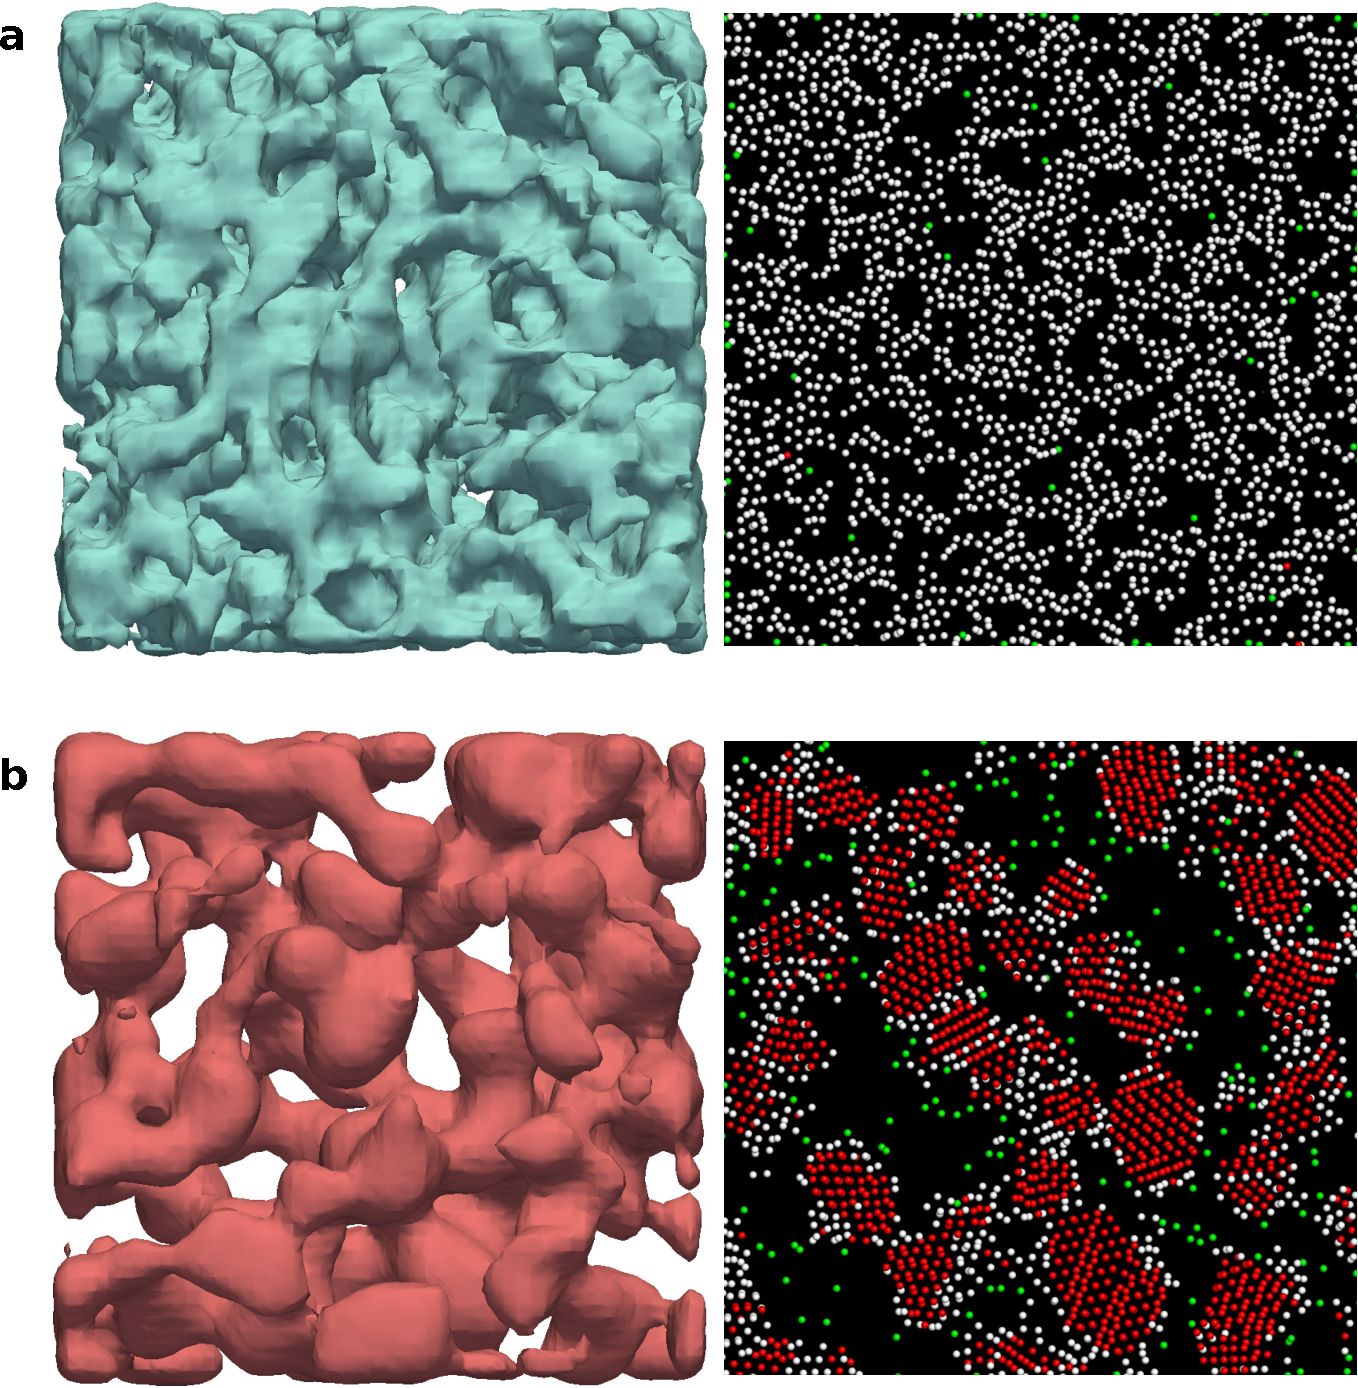
\includegraphics[height=11\baselineskip,clip=true,trim=0.5cm 0 0 0]{nature/fig2.pdf}
	
	\bigskip
	Compact structure and higher local $\phi$ \alert{because crystallized}
\end{frame}

\begin{frame}{Another class of gel? Crystal-gel?}
	\begin{itemize}
	\item Phase separation arrested by crystallisation
	\begin{description}
		\item[polymer blend] Tanaka \& Nishi \textit{PRL} 1985
		\item[simulations] Soga \textit{J.Chem. Phys.} 1999; Fortini \textit{PRE} 2008 
	\end{description}
	\item Spinodal then crystallisation
	\begin{description}
		\item[simulations] Pérez \textit{Langmuir} 2011
		\item[microgravity] (triple coexistence) Sabin \textit{PRL} 2012
	\end{description}
	\end{itemize}
	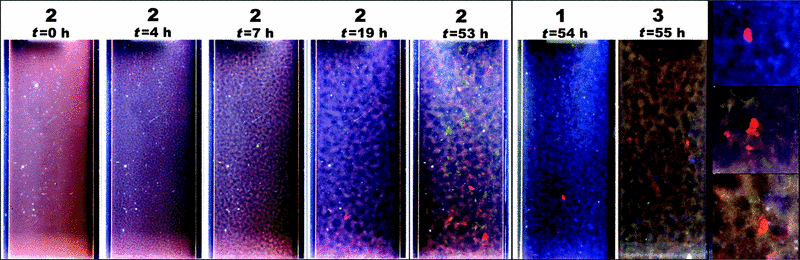
\includegraphics[width=\textwidth]{presentation/micrograv_Sabin2012}
\end{frame}

\begin{frame}{Crystals outgrow metastable liquid}
	\vspace{\baselineskip}
	\tikzsetnextfilename{crystal_fates}%
	\begin{tikzpicture}
	\begin{groupplot}[%
				group style={
					group name=g, group size=2 by 1,
					horizontal sep=4em,
					},
			width=0.5\linewidth,
			%height=0.5\linewidth,
			xlabel absolute, every axis x label/.append style={anchor=base, font=\footnotesize, yshift=-0.5em},
		]
		\nextgroupplot[
			title={nuclei},
			xlabel={$t/10^3\tau_B$}, ylabel=\#,
			xmin=0, xmax=13.0, ymin=0,
			no marks,
			legend style={cells={anchor=base west}},
			]
		\addplot table[x expr={\thisrowno{0}/2.3e3}]{data/fig3a_1.dat} node[left] at (rel axis cs:1,0.2) {avg size};
		\addplot table[x expr={\thisrowno{0}/2.3e3}]{data/fig3a_2.dat} node[left] at (rel axis cs:1,0.6) {number};
		%\legend{average size, average number};
	
		\nextgroupplot[
			title={cluster size distribution},
			xlabel={$s$}, ylabel=$R_g/\sigma$,
			xmode=log, ymode=log,
			ytick={0.5, 1, 2, 4}, yticklabels={$\frac{1}{2}$, 1, 2, 4},
			domain=1:5e2,
			]
		\addplot[only marks, red, thick, mark=*] file{data/fig3d_sqrt_1.dat};
		\addplot[black, ultra thick] {0.522*x^(1/3)} node[below left] at (axis cs:9e2,2.5) {$D=3$};
		\addplot[gray, ultra thick] {0.426*x^(1/2.53)} node[pos=0.08,below right] {$D=2.53$};
	\end{groupplot}
	\end{tikzpicture}
	
	\hfill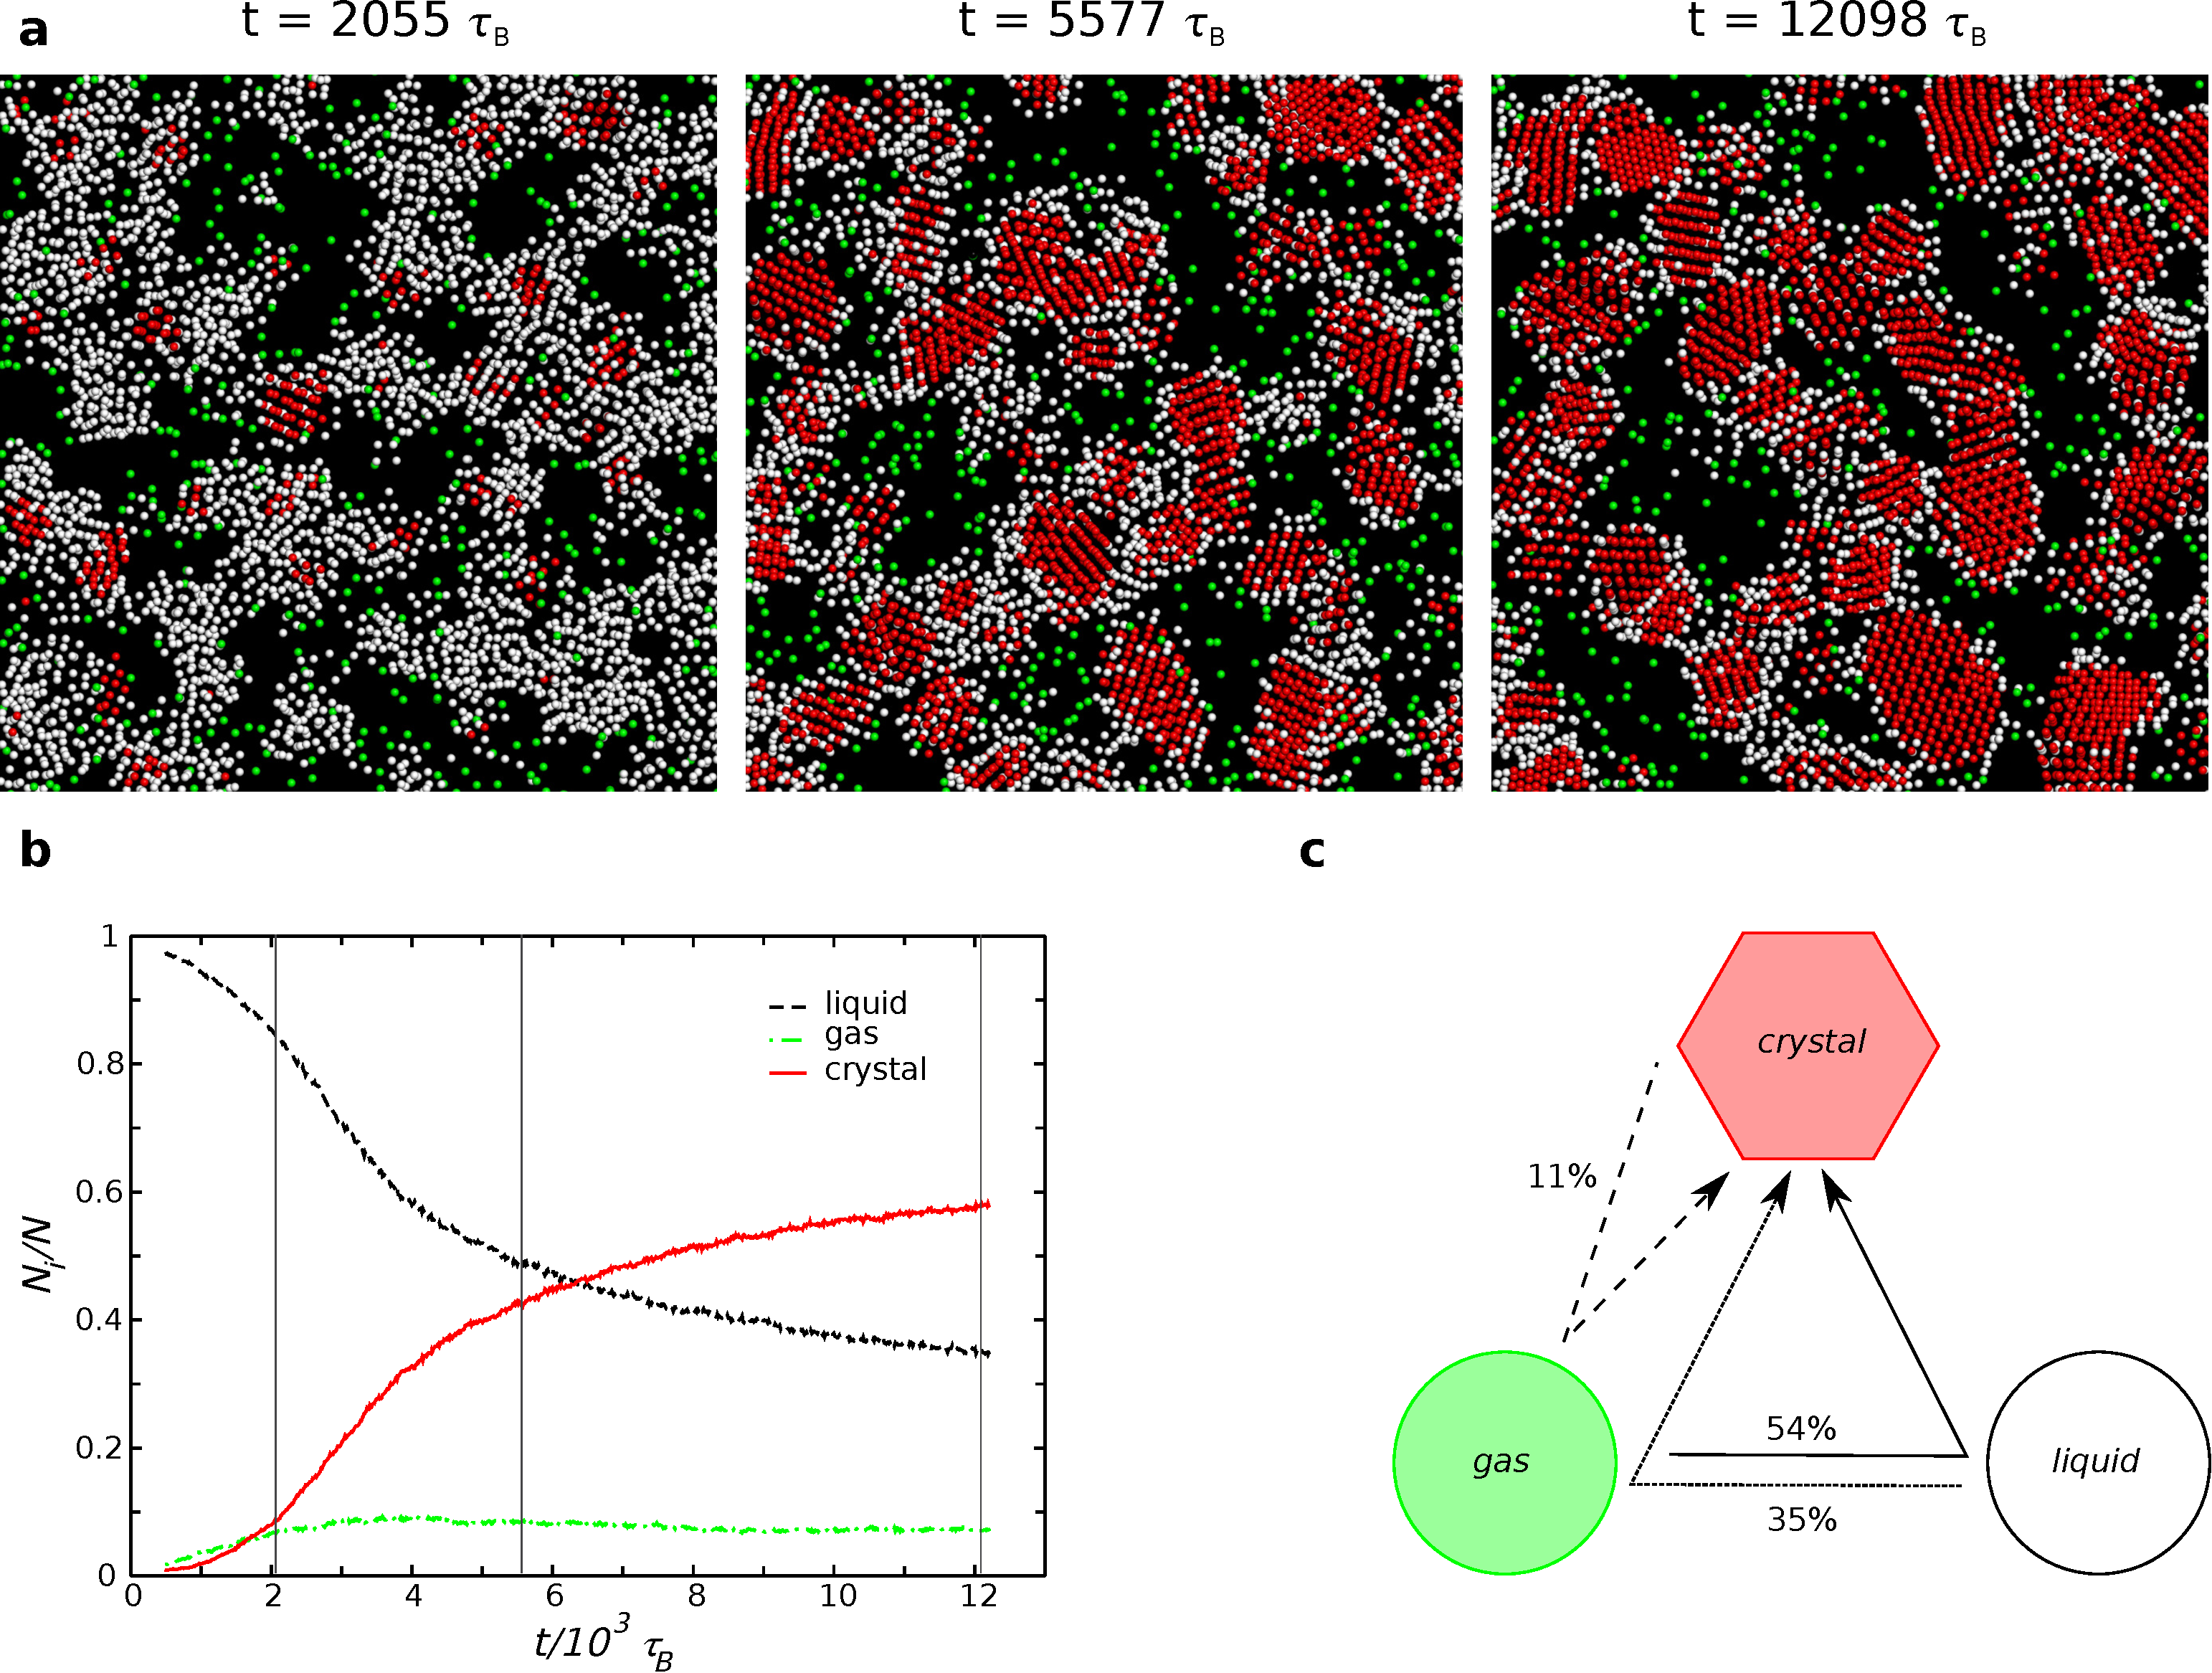
\includegraphics[width=0.95\textwidth, clip=true, trim=0 20cm 0 0]{nature/fig4.pdf}\hfill
\end{frame}


\begin{frame}{Dynamics: Bergeron > Ostwald}
	\vspace{\baselineskip}
	\begin{center}
	\tikzsetnextfilename{pathsX}\vspace{-0.5em}
\colorlet{gas}{green!40}
\colorlet{crystal}{red}


\begin{tikzpicture}[y=0.00105\textwidth, x=0.00105\textwidth, inner sep=0pt, outer sep=0pt]
      \path[fill=gas] (249.4278, 145.9555) .. controls (255.8399, 162.9241) and
        (255.6486, 150.9134) .. (264.1197,166.7770) .. controls (271.7753,178.4149) and
        (284.1357,186.0038) .. (291.3580,198.1149) .. controls (299.2358,208.4225) and
        (308.8596,217.6139) .. (319.2071,225.4715) .. controls (329.6855,232.4196) and
        (339.6264,240.5125) .. (351.8380,244.1310) .. controls (361.4203,248.1022) and
        (370.7233,252.7078) .. (380.1367,256.9895) .. controls (391.4156,260.4022) and
        (403.3859,258.7125) .. (414.9487,258.6726) .. controls (425.7231,254.4977) and
        (432.9781,243.8537) .. (439.4290,234.7953) .. controls (451.7800,217.5436) and
        (458.2006,197.1440) .. (466.2122,177.7904) .. controls (471.6441,149.0314) and
        (495.5153, 147.6479) .. (498.2319,145.8515) .. controls (410.7207,146.0915) and
        (337.0032,145.8879) .. (249.4278,145.9555) -- cycle;
      \path[fill=gas] (561.4952,145.9035) .. controls (561.4952,145.9035) and
        (549.0258,141.8419) .. (542.4009,151.7643) .. controls (535.6582,162.2127) and
        (532.5285,174.0012) .. (524.9087,183.7558) .. controls (516.5996,196.1379) and
        (517.0059,212.0197) .. (506.7764,223.0120) .. controls (497.1343,232.9443) and
        (487.3188,242.6413) .. (476.8068,251.5109) .. controls (469.0123,261.5858) and
        (459.0759,270.7573) .. (457.1823,283.9613) .. controls (452.8893,297.5050) and
        (448.7808,312.9003) .. (454.1515,326.4042) .. controls (461.6885,336.9556) and
        (468.3435,349.2697) .. (479.5852,356.2220) .. controls (489.8740,362.1413) and
        (499.4121,368.7102) .. (508.7209,375.9653) .. controls (518.9046,379.5965) and
        (525.5886,387.1594) .. (529.5609,396.7014) .. controls (536.7327,406.6964) and
        (538.9936,419.1112) .. (546.3895,428.9986) .. controls (555.0208,437.3780) and
        (554.1097,438.9583) .. (561.4952,441.4922) -- cycle;
      \path[fill=gas] (498.4097,440.9035) .. controls (498.4097,440.9035) and
        (498.9997,444.1080) .. (494.7970,432.0881) .. controls (483.0387,415.8571) and
        (472.2338,398.4146) .. (457.1778,384.9720) .. controls (445.6967,377.7219) and
        (435.2272,368.2044) .. (421.6726,365.0475) .. controls (410.7197,359.6698) and
        (400.5448,353.9104) .. (390.9725,346.4716) .. controls (374.2105,338.8403) and
        (366.8647,320.9238) .. (354.0066,308.8500) .. controls (339.3442,293.5472) and
        (320.5199,281.6364) .. (299.5907,277.2060) .. controls (280.7665,269.0422) and
        (260.9918,278.6076) .. (243.0003,284.3880) .. controls (232.5837,289.8481) and
        (224.8066,299.2918) .. (213.4444,303.0482) -- (180,324.8903) -- (180,440.9035) -- cycle;
      \path[fill=gas] (180.5052,262.5020) .. controls (180,262.5020) and
        (224.0280,240.9675) .. (242.9564,225.5882) .. controls (251.5564,212.9283) and
        (251.1938,196.9087) .. (250.5459,182.2558) .. controls (248.0335,166.2656) and
        (235.6552,158.2869) .. (223.2013,149.0965) .. controls (212.6095,142.9380) and
        (203.6451,145.9035) .. (203.6451,145.9035) -- (180,145.9035) -- cycle;
	\fill[crystal] (274.8619,237.0951) circle (17);
	\fill[crystal] (406.1129,300) circle (31) node[black] {crystal};
	\fill[crystal] (497.3412,397) circle (16);
	\fill[crystal] (498,175) circle (20);
	\fill[crystal] (317,250) circle (16);
	%phases
    \node[anchor=west, inner sep=0] at (200,400) {gas};
    \node[anchor=west, inner sep=0] at (180,270){liquid};


	  \begin{scope}[xshift=0.5\textwidth]
    \path[fill=green!40] (245.4278,145.9555) .. controls (251.8399,162.9241) and
      (249.6486,150.9134) .. (258.1197,166.7770) .. controls (265.7753,178.4149) and
      (278.1357,186.0038) .. (285.3580,198.1149) .. controls (293.2358,208.4225) and
      (308.8596,217.6139) .. (319.2071,225.4715) .. controls (329.6855,232.4197) and
      (339.6264,246.5126) .. (351.8380,250.1310) .. controls (361.4203,254.1022) and
      (370.7233,258.7078) .. (380.1367,262.9895) .. controls (391.4156,266.4022) and
      (403.3859,264.7125) .. (414.9487,264.6726) .. controls (425.7231,260.4977) and
      (438.9781,243.8537) .. (445.4290,234.7954) .. controls (457.7800,217.5436) and
      (460.2006,197.1441) .. (468.2122,177.7904) .. controls (469.3721,163.6755) and
      (481.4553,151.1804) .. (496.2319,145.8515) .. controls (408.7207,146.0916) and
      (333.0032,145.8879) .. (245.4278,145.9555) -- cycle;
    \path[fill=gas] (561.4952,145.9035) .. controls (561.4952,145.9035) and
      (543.0258,141.8419) .. (536.4009,151.7643) .. controls (529.6582,162.2127) and
      (526.5285,174.0012) .. (518.9087,183.7558) .. controls (510.5996,196.1379) and
      (511.0059,212.0197) .. (500.7764,223.0120) .. controls (491.1343,232.9443) and
      (481.3188,242.6413) .. (470.8068,251.5109) .. controls (463.0123,261.5858) and
      (453.0759,270.7573) .. (451.1823,283.9613) .. controls (446.8893,297.5050) and
      (442.7808,312.9003) .. (448.1515,326.4042) .. controls (455.6885,336.9556) and
      (462.3435,349.2697) .. (473.5852,356.2219) .. controls (483.8740,362.1413) and
      (493.4121,368.7102) .. (502.7209,375.9653) .. controls (512.9046,379.5965) and
      (525.5886,387.1594) .. (529.5609,396.7014) .. controls (536.7327,406.6964) and
      (532.9936,419.1112) .. (540.3895,428.9986) .. controls (550.1481,437.0509) and
      (554.6509,439.1440) .. (561.4952,441.4922) -- cycle;
    \path[fill=gas] (504.4097,440.9035) .. controls (504.4097,440.9035) and
      (504.9997,444.1080) .. (500.7970,432.0882) .. controls (489.0387,415.8571) and
      (478.2338,398.4147) .. (463.1778,384.9720) .. controls (451.6967,377.7220) and
      (445.2272,364.2044) .. (431.6726,361.0475) .. controls (420.7197,355.6698) and
      (406.5448,353.9104) .. (396.9725,346.4716) .. controls (380.2105,338.8403) and
      (376.8647,316.9238) .. (364.0066,304.8500) .. controls (349.3442,289.5472) and
      (324.5199,277.6364) .. (303.5907,273.2061) .. controls (284.7665,265.0423) and
      (260.9918,262.6076) .. (243.0003,268.3880) .. controls (232.5837,273.8481) and
      (224.8066,283.2918) .. (213.4444,287.0482) -- (180,308.8903) -- (180,440.9035) -- cycle;
    \path[fill=gas] (180.5052,278.5020) .. controls (180,278.5020) and
      (224.0280,256.9675) .. (242.9564,241.5882) .. controls (251.5564,228.9283) and
      (257.1938,196.9087) .. (256.5460,182.2558) .. controls (254.0335,166.2656) and
      (241.6552,158.0939) .. (229.2013,148.9035) .. controls (218.6095,142.7450) and
      (209.6446,145.9035) .. (209.6446,145.9035) -- (180,145.9035) -- cycle;
	\fill[crystal] (274.8619,237.0951) circle (35) coordinate(ca);
	\fill[crystal] (406.1129,300) circle (62) +(0,-31) coordinate(cb) +(-10,31) coordinate(cbb);
	\fill[crystal] (497.3412,397) circle (40) coordinate(cc);
	\fill[crystal] (498,175) circle (20) coordinate(cd);
	\fill[crystal] (317,250) circle (32) ++(10,-15) coordinate(ce);
	%processes
	\node[anchor=east] at (561,260) (direct) {Direct};
	\draw[->, very thick] (direct) to[bend right, distance=15] (cd);
	\draw[->, very thick, dotted] (200,280) coordinate (l) to[out=70, in=130, distance=30] (cbb);
	\draw[->, very thick, dashed] (ce) to[out=-60, in=-90, distance=25] (cb);
  \node[below] at ($(ce)!0.8!-60:(cb)$) {Ostwald};
  \node[above] at ($(l)!0.65!30:(cbb)$) {Bergeron};
  \end{scope}
\end{tikzpicture}

	\end{center}
	\begin{columns}
	\column{0.5\textwidth}
	\begin{itemize}
	\item Individual trajectories
	\item Probability of path to X
	\end{itemize}
	\column{0.5\textwidth}
	\tikzsetnextfilename{pathsX2}%
	\begin{tikzpicture}
	\node[regular polygon, regular polygon sides=3, minimum width=5em] (tri){};
	\node[circle, minimum width=3.5em, fill=green!40, left=1em of tri.corner 2] (gas) {gas};
	\node[circle, minimum width=3.5em, draw, fill=white, right =1em of tri.corner 3] (liq) {liquid};
	\node[regular polygon, regular polygon sides=6, fill=red,minimum width=3.5em, inner sep=0, above=0 of tri.corner 1] (X) {crystal};
	\draw[->, very thick] ($(tri.corner 2)+(0,0.25em)$) -- ($(liq.west)+(0,0.25em)$) node[midway, above]{54\%}-- (X);
	\draw[->, very thick, dotted] ($(tri.corner 3)+(0,-0.25em)$) -- ($(gas.east)+(0,-0.25em)$) node[midway, below]{35\%}-- (X);
	\draw[->, very thick, dashed] (X) edge [in=190,out=-130,loop] node[left]{11\%} ();
	\end{tikzpicture}
	\end{columns}
\end{frame}

\begin{frame}{Conclusion}
	\begin{itemize}
		\item A particle level colloidal analogue to the Bergeron process
		\item Generic "crystal-gel" process
		\begin{enumerate}
			\item gas-liquid phase separation below melting point
		of a crystal
			\item weak or little frustration against crystallization
			\item dynamical slowing down in a supercooled liquid state
			\begin{itemize}
				\item viscoelastic phase separation
				\item network of the minority liquid phase
			\end{itemize}
			\item low supercooling: crystallisation > vitrification
		\end{enumerate}
		\item Gels of poor glass formers (monoatomic systems)
		\item Porous material with a large area of crystalline planes
		\begin{itemize}
			\item catalysis, sensing, filtration, super-capacitor\ldots
			\item single step
		\end{itemize}
	\end{itemize}
\end{frame}

\appendix
\newcounter{finalframe}
\setcounter{finalframe}{\value{framenumber}}

\begin{frame}[plain]
\end{frame}

\begin{frame}{Reproducibility in capillary}
	\hfill $\phi\approx 0.33$, $c_P=\SI{0.40}{\milli\gram/\gram}$
	
	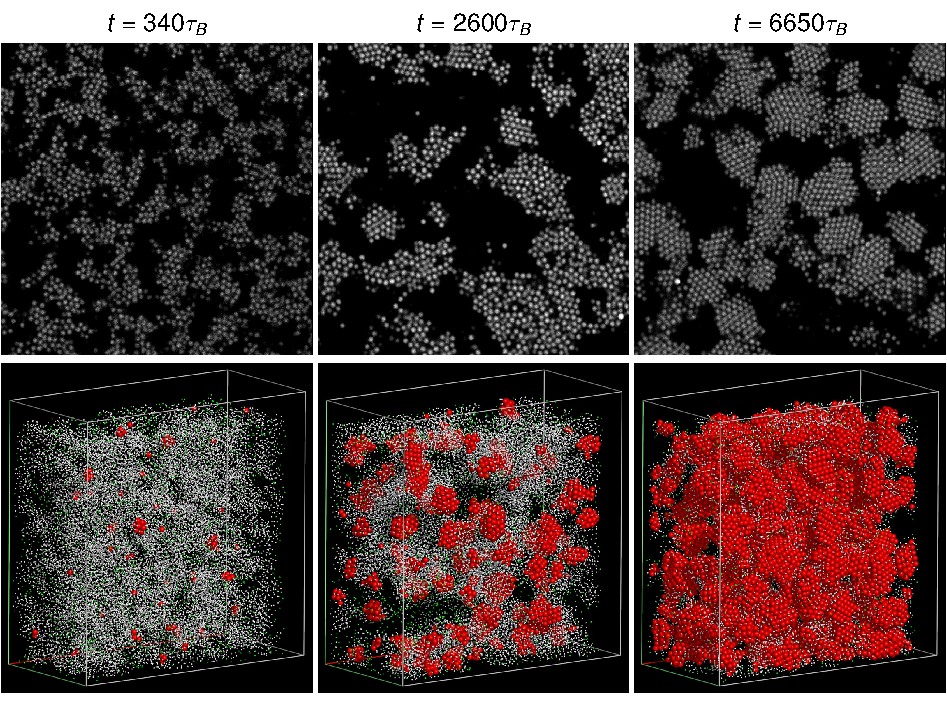
\includegraphics[width=\textwidth]{nature/capillary}
\end{frame}

\begin{frame}{Transition probabilities}
	\vspace{\baselineskip}
	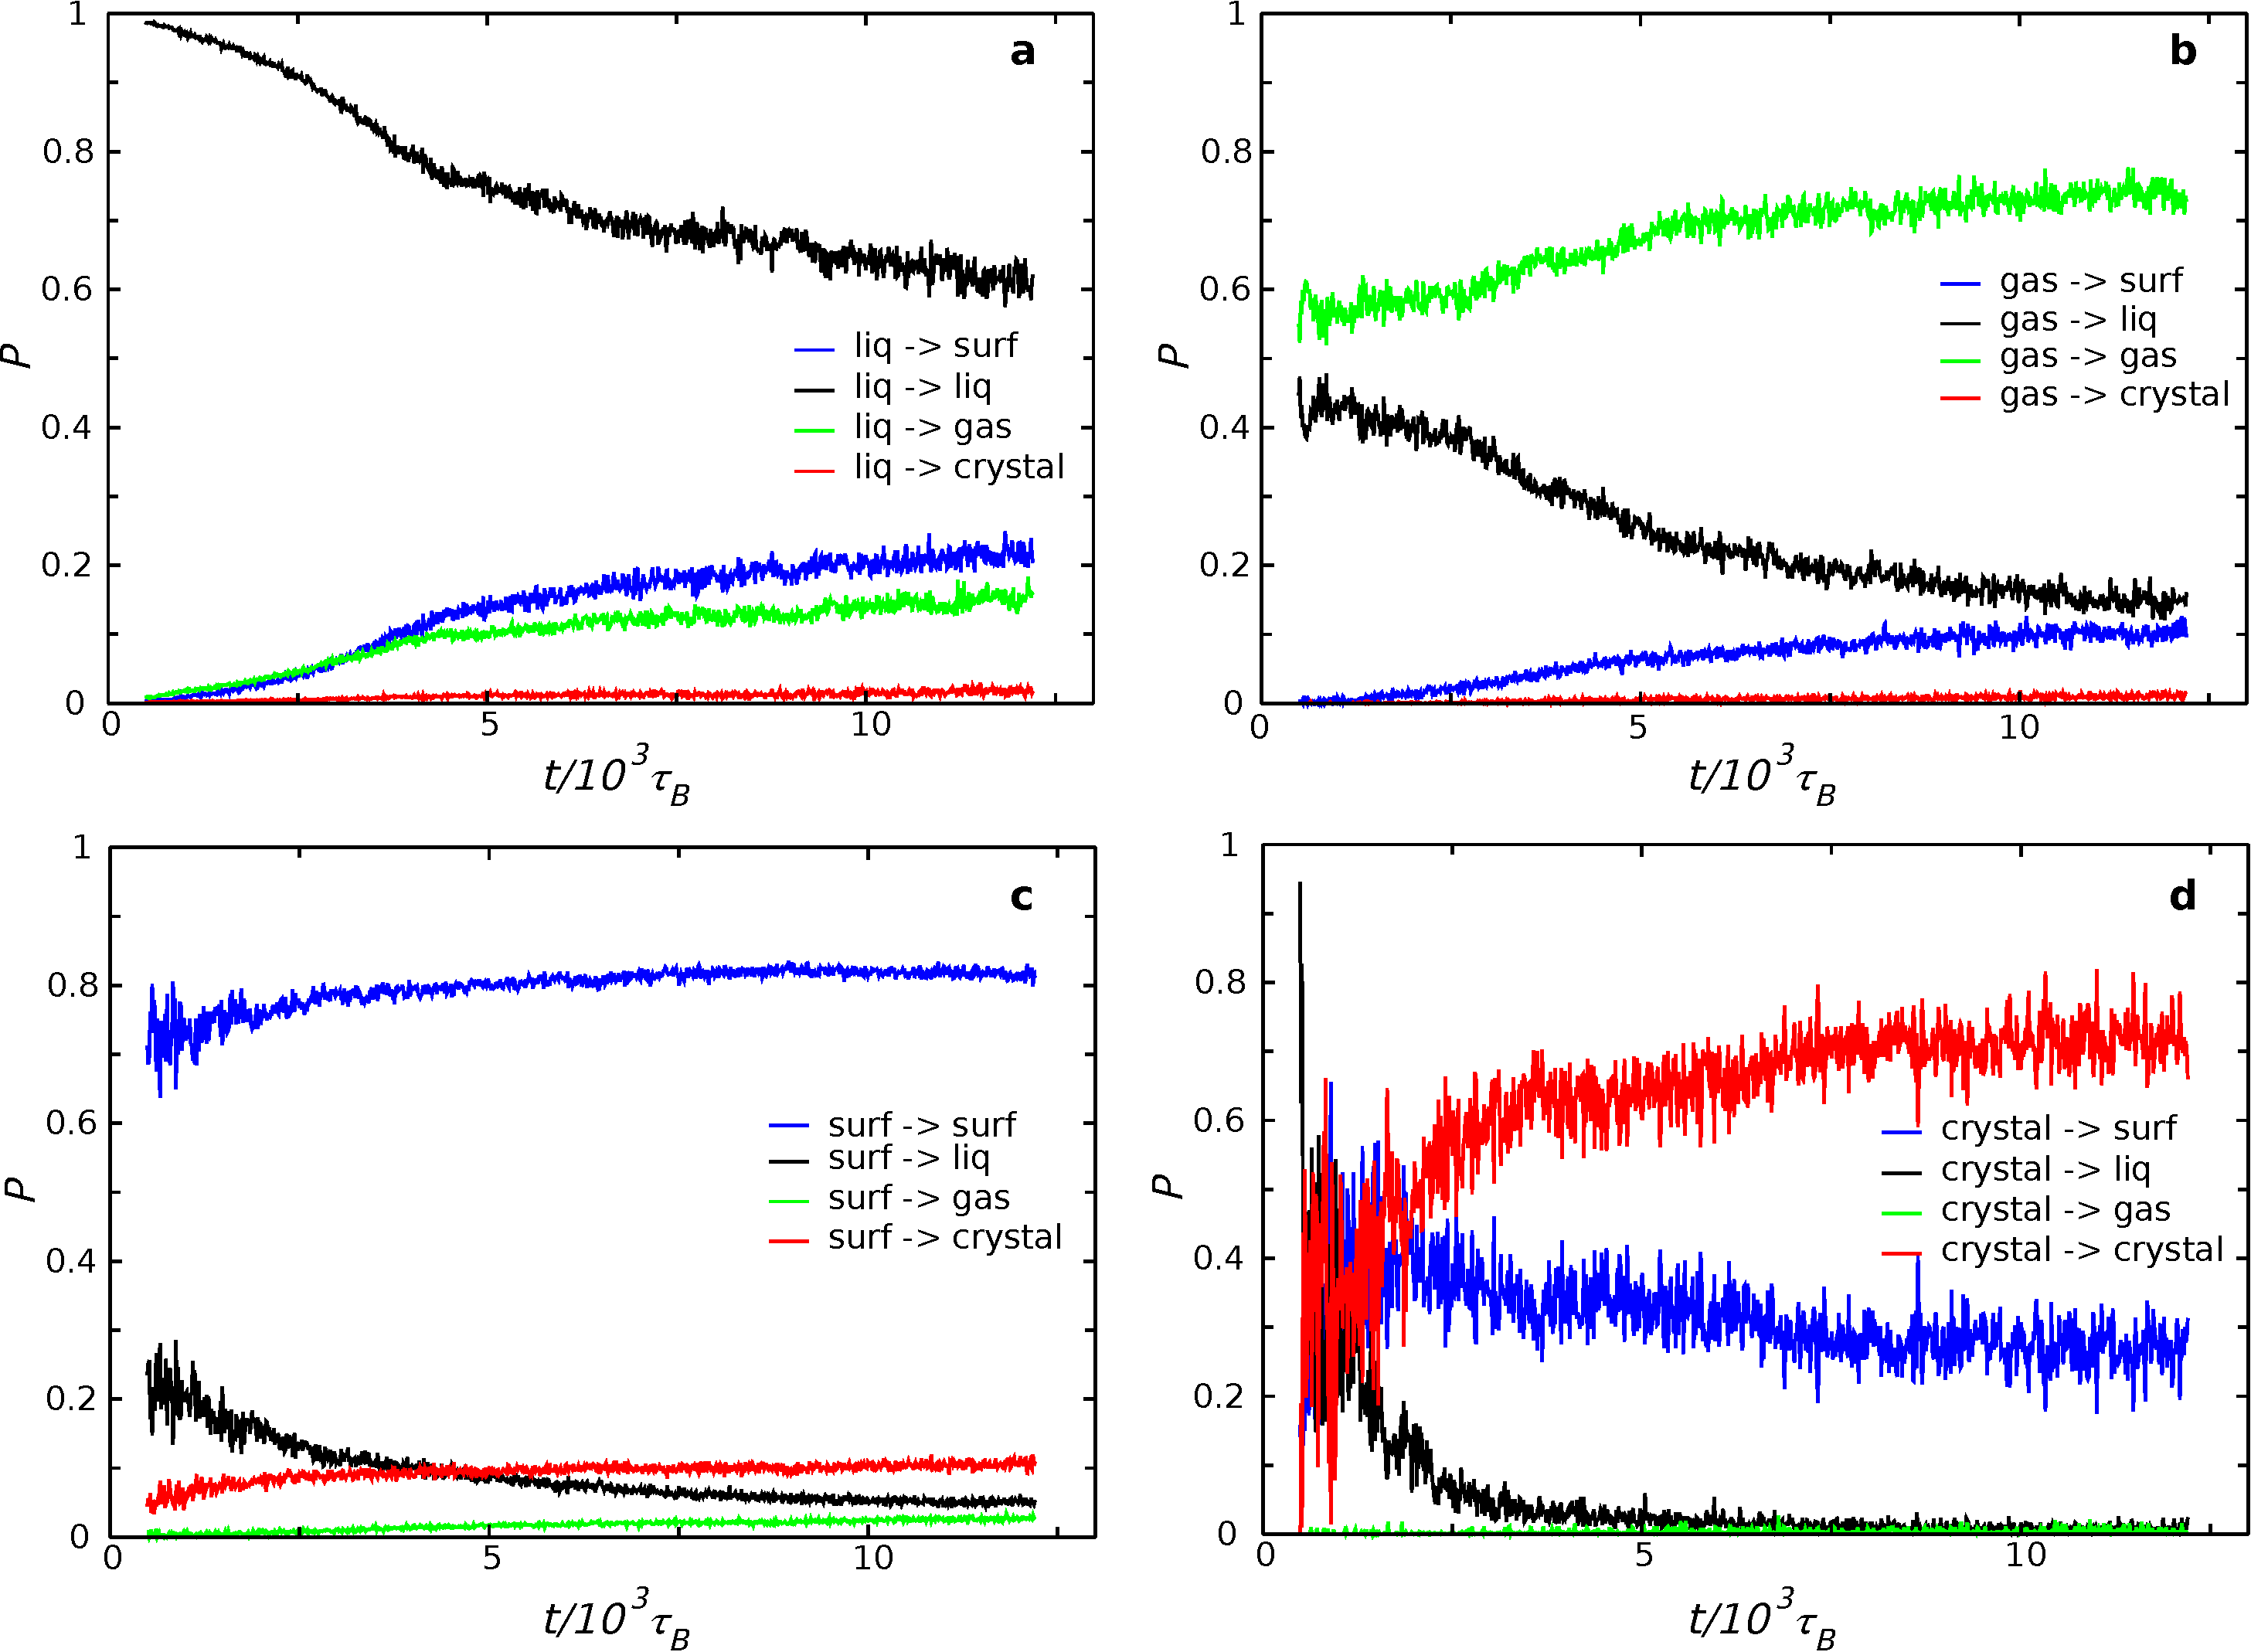
\includegraphics[width=\textwidth]{nature/sfig1.pdf}
\end{frame}

\begin{frame}{phase definition}
	\begin{description}
	\item[crystal]
		\begin{itemize} 
		\item particle $i$ has $N_b(i)=12$ neighbours
		\item $\displaystyle q_{6 m}(i)=\frac{1}{N_b(i)}\sum_{j=1}^{N_b(i)}
	Y_{6 m}(\mathbf{r_{ij}}),\quad -6 <m<6$
		\item crystalline bond $(i,j)$: \[(\mathbf{q}_{6}(i)/|\mathbf{q}_{6}(i)|)\cdot(\mathbf{q}_{6}(j)/|\mathbf{q}_{6}(j)|)>0.7\]
		\item crystalline particle: $7$ crystalline bonds
		\end{itemize}
	\item[surface] two neighbouring crystal particles
	\item[liquid] at least four neighbouring particles
	\item[gas]
	\end{description}
\end{frame}

\begin{frame}{Colloid and polymer sizes}
	Direct measurement \alert{too imprecise}
	\begin{itemize}
	\item diffusion constant $\Rightarrow R= \SI{2.3 +- 0.05}{\micro\metre}$
	\item Flory scaling litterature measurements $\Rightarrow R_g=\SI{76. +- 50.}{\nano\metre}$
	\end{itemize}
	
	\begin{block}{Adjusting theoretical and experimental phase diagrams}
	\begin{enumerate}
	\item to have the final local volume fraction of the 12-neighboured particles in the crystallising sample to be equal to the theoretical equilibrium crystal volume fraction 
	\item to have the theoretical spinodal line to correspond to the gel region boundary.
	\end{enumerate}
	\end{block}
	Starting from our initial estimates of $\sigma$ and $R$ we iteratively converge to $R=\SI{80}{\nano\metre}$, $\sigma = \SI{2.25}{\micro\metre}$ and a crystal (without defects) at $0.723$.
\end{frame}

\begin{frame}{Carnahan-Starling is not enough}
	\tikzsetnextfilename{CSphasediag}%
	\begin{tikzpicture}[
		every axis/.style={
			xlabel absolute, every axis x label/.append style={anchor=base, yshift=-0.5em},
			ylabel absolute, every axis y label/.append style={anchor=base, yshift=-0.5em}
			}]
		\pgfplotscreateplotcyclelist{samples}{%
		blue,mark=square*,\\%
		cyan,mark=square\\%
		red, thick, mark=*\\%
		red!65!yellow, mark=otimes\\%
		red!30!yellow, mark=oplus\\%
		red!65!black, mark=o\\%
		}%
		\begin{groupplot}[
			group style={
					group name=g, group size=2 by 2,
					horizontal sep=0.5em,
					vertical sep=0.5em,
					x descriptions at=edge bottom,
					y descriptions at=edge left,
				},
			cycle list name=samples,
			width=0.5\textwidth,
			%height=0.5\linewidth,
			axis on top,
			xlabel={$\phi$},
		]
		\nextgroupplot[
			ylabel={attraction},
			xmin=0,xmax=0.74,
			ymin=0, ymax=2400, %ytick={0,0.5,...,2},
			mark options={solid}
			]
			\begin{scope}[dotted, mark repeat=2,mark phase=2,<->]
		\addplot file {res_sample0.phd};
		\addplot file {res_sample1.phd};
		\addplot file {res_sample2.phd};
		\addplot file {res_sample3.phd};
		\addplot file {res_sample4.phd};
		\addplot file {res_sample5.phd};
		\end{scope}
			\addplot[black, dashed,no marks] file {res_gasliquid_sg.phd};% node[diamond, fill, inner sep=2pt] at (current plot begin){};
			\addplot[black, dashed,no marks] file {res_gasliquid_sl.phd};
			\addplot[black, no marks] file {res_gasliquid_bl.phd};
			\addplot[black, no marks] file {res_gasliquid_bg.phd};
			\addplot[fill=lightgray!50, no marks, draw=none] file {res_fluidcrystal_f.phd} -- (rel axis cs:0,0) \closedcycle;
			\addplot[fill=lightgray!50, no marks, draw=none] file {res_fluidcrystal_x.phd}  -| (rel axis cs:1,0) \closedcycle;

	\nextgroupplot[
			xmin=0,xmax=0.74,
			ymin=0, ymax=2400, %ytick={0,0.5,...,2},
			mark options={solid}
			]
			\begin{scope}[dotted, mark repeat=2,mark phase=2,<->]
		\addplot file {res_sample0.phd};
		\addplot file {res_sample1.phd};
		\addplot file {res_sample2.phd};
		\addplot file {res_sample3.phd};
		\addplot file {res_sample4.phd};
		\addplot file {res_sample5.phd};
		\end{scope}
			\addplot[black, dashed,no marks] file {res_gasliquidCS_sg.phd};% node[diamond, fill, inner sep=2pt] at (current plot begin){};
			\addplot[black, dashed,no marks] file {res_gasliquidCS_sl.phd};
			\addplot[black, no marks,skip coords between index={10}{100}] file {res_gasliquidCS_bl.phd};
			\addplot[black, no marks,skip coords between index={10}{100}] file {res_gasliquidCS_bg.phd};
			\addplot[fill=lightgray!50, no marks, draw=none] file {res_fluidcrystal_f.phd} -- (rel axis cs:0,0) \closedcycle;
			\addplot[fill=lightgray!50, no marks, draw=none] file {res_fluidcrystal_x.phd}  -| (rel axis cs:1,0) \closedcycle;

		\nextgroupplot[
			ylabel={P concentr. (\si{\milli\gram/\gram})},
			xmin=0,xmax=0.74,
			ymin=0, ymax=1.9, ytick={0,0.5,...,2},
			mark options={solid}
			]
			\begin{scope}[dotted, mark repeat=2,mark phase=2,<->]
			\addplot file {sample0.phd};
			\addplot file {sample1.phd};
			\addplot file {sample2.phd};
			\addplot file {sample3.phd};
			\addplot file {sample4.phd};
			\addplot file {sample5.phd};
			\end{scope}
			\addplot[black, dashed,no marks] file {gasliquid_sg.phd};% node[diamond, fill, inner sep=2pt] at (current plot begin){};
			\addplot[black, dashed,no marks] file {gasliquid_sl.phd};
			\addplot[black, no marks] file {gasliquid_bl.phd};
			\addplot[black, no marks] file {gasliquid_bg.phd};
			\addplot[fill=lightgray!50, no marks, draw=none] file {fluidcrystal_f.phd} -- (rel axis cs:0,0) \closedcycle;
			\addplot[fill=lightgray!50, no marks, draw=none] file {fluidcrystal_x.phd}  -| (rel axis cs:1,0) \closedcycle;
			\addplot[only marks, mark=triangle] file{fluid_samples.phd};
		
		\nextgroupplot[
			xmin=0,xmax=0.74,
			ymin=0, ymax=1.9, ytick={0,0.5,...,2},
			mark options={solid}
			]
			\begin{scope}[dotted, mark repeat=2,mark phase=2,<->]
			\addplot file {sample0.phd};
			\addplot file {sample1.phd};
			\addplot file {sample2.phd};
			\addplot file {sample3.phd};
			\addplot file {sample4.phd};
			\addplot file {sample5.phd};
			\end{scope}
			\addplot[black, dashed,no marks] file {gasliquidCS_sg.phd};% node[diamond, fill, inner sep=2pt] at (current plot begin){};
			\addplot[black, dashed,no marks] file {gasliquidCS_sl.phd};
			\addplot[black, no marks,skip coords between index={10}{100}] file {gasliquidCS_bl.phd};
			\addplot[black, no marks,skip coords between index={10}{100}] file {gasliquidCS_bg.phd};
			\addplot[fill=lightgray!50, no marks, draw=none] file {fluidcrystal_f.phd} -- (rel axis cs:0,0) \closedcycle;
			\addplot[fill=lightgray!50, no marks, draw=none] file {fluidcrystal_x.phd}  -| (rel axis cs:1,0) \closedcycle;
			\addplot[only marks, mark=triangle] file{fluid_samples.phd};
	\end{groupplot}
	\end{tikzpicture}
\end{frame}

\setcounter{framenumber}{\value{finalframe}}
\end{document}

